\chapter{Специальная часть}
\section{Постановка задачи}
\label{sec:spec:ProblemDefinition}
Разработать метод мониторинга состояния ЛА по данным телеметрии на основе методов интеллектуального анализа данных. Реализовать программную систему для ПЭВМ, использующую данный метод.

Система должна удовлетворять следующим требованиям:
\begin{itemize}
	\item строить модель объекта контроля (ОК) только на основе телеметрии при различных режимах его работы, без априорных данных о предметной области, его назначении, составе, конструкции (обучение без учителя);
	\item обладать способностью классифицировать аномалии в работе ОК;
	\item в случае, если текущее поведение ОК не было представлено в обучающей выборке, давать оператору численную характеристику отклонения ОК от номинальных режимов;
	\item обрабатывать большие массивы входных данных (несколько десятков тысяч точек) за конечное время;
	\item учитывать как непрерывные, так и дискретные параметры ОК;
	\item не иметь ограничений на закон распределения входных данных;
	\item быть устойчивой к аномалиям в обучающей выборке;
	\item быть устойчивой к отсутствию значений каких-либо параметров во входных данных;
	\item определять состояние ОК в режиме реального времени.
\end{itemize}

\section{Анализ существующих методов выявления аномалий без учителя}
На данный момент существует несколько методов, для которых доказана возможность применения их в системах контроля состояния ЛА. Такими методами являются Orca, GritBot, модель гауссовых смесей (Gaussian Mixture Model, GMM), динамические байесовские сети (Dynamic Bayesian Network, DBN), одноклассовый метод опорных векторов (One-Class Support Vector Machine, SVM) и IMS (Inductive Monitoring System)~\cite{MartinCompUnsupervisedDetectionMethods}.

\subsection{Orca}
Orca~---~метод поиска аномалий без учителя, использующий подход «ближайшего соседа» (nearest neighbor) для поиска аномалий~\cite{SchwabacherMachLearnAppl}. Данный метод был разработан Стефеном Бэйем (Institute for the Study of Learning and Expertise) и Марком Швабахером (NASA Ames Research Center) и подробно описан в~\cite{BaySchwabacherOrca}. Orca относится к методам обнаружения аномалий, основанных на измерении расстояний между точками (distance-based).

Понятие аномалии для данного класса методов определено следующим образом: «объект $O$ в выборке $T$ является аномалией, если по крайней мере доля $p$ из всех объектов в $T$ лежит дальше от $O$, чем расстояние $D$»~\cite{KnorrNgDistBasedAlgorithms}. Distance-based методы являются обобщением некоторых статистических тестов на аномальность. Данный класс методов не требует априорных знаний о виде распределения для выборки. Кнорр и Нг предложили простейший алгоритм на вложенных циклах (Nested Loop, NL)~\cite{KnorrNgDistBasedAlgorithms}, который находит аномалии путём вычисления расстояния между всеми точками в исходной выборке. Сложность данного алгоритма составляет $O(kN^2)$, где $k$ --- размерность пространства, а $N$ --- размер выборки.

Несмотря на то, что были разработаны более эффективные c т.з. вычислительной сложности алгоритмы (\cite{TaoMiningDistBasedOutliersFromLargeDB}~и~\cite{AngiulliVeryEfficientMiningDistBasedOutliers}), на практике наиболее сложным является определение расстояния $D$, по достижению которого точку следует считать аномалией. Может потребоваться непредсказуемо большое число итераций, чтобы найти подходящее значение $D$. Найти интервал $[D_{min}, D_{max}]$ возможно путём полного перебора, как показано в~\cite{TaoMiningDistBasedOutliersFromLargeDB}, но данный подход обладает слишком высокой вычислительной сложностью.

В качестве решения данной проблемы было предложено следующее определение аномалии, не требующее задания $D$: «объект считается аномалией, если это один из $n$ объектов с наибольшим расстоянием до их $k$-ых ближайших соседей, где~$k,n\in\mathbb{N}$»~\cite{RamaswamyEffAlgoMiningOutliers}. Пользователю достаточно указать количество аномалий, которое должен вернуть алгоритм, без прямого указания дистанции $D$. Более того, возвращаемые алгоритмом аномалии будут ранжированы по степени аномальности, являющейся численной характеристикой.

Orca использует данный подход, развивая идею алгоритма на вложенных циклах~(NL). Данный алгоритм на больших массивах данных показывает сложность, близкую к линейной~\cite{BaySchwabacherOrca}.

Псевдокод алгоритма приведён в листинге~\ref{lst:spec:OrcaPseudocode}. Ключевыми особенностями алгоритма являются:
\begin{itemize}
	\item необходимость рандомизации исходных данных (строка~\ref{lst:spec:OrcaPseudocode:Random}). Для эффективной работы алгоритма требуется, чтобы объекты в выборке находились в случайном порядке. При обработке выборки на ПЗУ возможно рандомизировать выборку за линейное время и используя конечный объём памяти~\cite{BaySchwabacherOrca};
	\item использование вложенных циклов (строка~\ref{lst:spec:OrcaPseudocode:NL}). Основной идеей является отслеживание ближайших соседей для каждого объекта в $D$;
	\item правило отсечения (строка~\ref{lst:spec:OrcaPseudocode:Pruning}). Когда для ближайших соседей объекта степень аномальности становится меньше, чем величина среза, алгоритм удаляет данный объект, так как больше нет оснований считать его аномальным. Чем больше объектов перебирает алгоритм, тем выше становится величина среза, улучшая таким образом эффективность алгоритма по времени.
\end{itemize}

\begin{algorithm}[h]
\caption{Псевдокод алгоритма Orca}
\label{lst:spec:OrcaPseudocode}
\begin{algorithmic}[1]
\REQUIRE $k$, количество ближайших соседей; $n$, количество аномалий; $D$, выборка.
\ENSURE $O$, множество аномалий
\STATE Перемешать все объекты в выборке $D$. \label{lst:spec:OrcaPseudocode:Random}
\STATE Инициализировать величину среза нулём.
\WHILE{в выборке $D$ остались необработанные объекты}
	\STATE Загрузить фиксированное количество объектов $B$ в буфер.
	\FOR{каждого объекта $d$ в $D$} \label{lst:spec:OrcaPseudocode:NL}
		\FOR{каждого объекта $b$ в $B$}
			\STATE Вычислить расстояние между $b$ и $d$.
			\IF{$d$ ближе к $b$, чем $k$ ближайших соседей $b$}
				\STATE Заменить соседа с наибольшим расстоянием на $d$.
				\STATE Вычислить степень аномальности $b$.
				\IF{степень аномальности ниже величины среза} \label{lst:spec:OrcaPseudocode:Pruning}
					\STATE Удалить $b$ из $B$.
				\ENDIF
			\ENDIF
		\ENDFOR
	\ENDFOR
	\STATE Поместить в $O$ оставшиеся в $B$ объекты.
	\STATE Отсортировать объекты в $O$ по степени аномальности.
	\STATE Оставить в $O$ только $n$ объектов.
	\STATE Обновить величину среза степенью аномальности последнего объекта в $O$.
\ENDWHILE
\RETURN $O$.
\end{algorithmic}
\end{algorithm}

Преимуществами метода являются:
\begin{itemize}
	\item превосходная масштабируемость: на выборках большого объёма производительность алгоритма близка к линейной;
	\item низкие требования к памяти: не требуется загружать в память всю выборку;
	\item возможность задать любую метрику для расстояния и функцию для определения степени аномальности.
\end{itemize}

Недостатки следуют из природы метода. В качестве основных можно выделить следующие:
\begin{itemize}
	\item в худшем случае (например, когда выборка не содержит аномалий) производительность алгоритма крайне низкая. Из-за вложенных циклов может потребоваться $O(N^2)$ операций вычисления расстояния и $O(N/l \cdot N)$ операций доступа к данным, где $l$ --- размер буфера;
	\item в качестве результата алгоритм возвращает фиксированное число аномалий, указанное перед началом работы.
\end{itemize}

\subsection{GritBot}
GritBot является коммерческим продуктом компании RuleQuest Research~\cite{GritBotWebPage}. Вместо поиска точек, наиболее сильно отличающихся от остальной выборки, данный метод ищет подмножества, аномальность которых очевидна~\cite{SchwabacherMachLearnAppl}. Метод определяет границы для непрерывных и список возможных значений для дискретных переменных, формируя набор правил классификации. GritBot основан на использовании деревьев решений~\cite{MartinCompUnsupervisedDetectionMethods} и использует алгоритм C4.5~\cite{MLInCyberTrust}, разработанный Джоном Квинланом и описанный им в~\cite{QuinlanC45}.

Для того, чтобы с помощью C4.5 построить дерево решений и применять его, входные данные должны удовлетворять нескольким условиям.

Информация об объектах, которые необходимо классифицировать, должна быть представлена в виде конечного набора признаков (атрибутов), каждый из которых имеет дискретное или непрерывное значение. Такой набор атрибутов называется \textit{примером}. Для всех примеров количество атрибутов и их состав должны быть постоянными.

Множество классов, на которые будут разбиваться примеры, должно иметь конечное число элементов, а каждый пример должен однозначно относиться к конкретному классу. Для случаев с нечёткой логикой, когда примеры принадлежат к классу с некоторой вероятностью, C4.5 неприменим.

В обучающей выборке количество примеров должно быть значительно больше количества классов, к тому же каждый пример должен быть заранее ассоциирован со своим классом. По этой причине C4.5 является вариантом машинного обучения с учителем.

Данный алгоритм рекурсивно разбивает множество объектов на подмножества так, чтобы энтропия полученных подмножеств была минимальна. Лучшее разбиение при этом выбираетя перебором всех возможных вариантов. 

Построение дерева решений в алгоритме C4.5 происходит следующим образом. Пусть имеется $T$ --- обучающая выборка примеров, а $C$ --- множество классов, состоящее из $k$ элементов. Для каждого примера из $T$ известна его принадлежность к какому-либо из классов $C_1\dots C_k$.

На первом шаге имеется корень и ассоциированное с ним множество $T$, которое необходимо разбить на подмножества. Для этого необходимо выбрать один из атрибутов в качестве проверки. Выбранный атрибут $A$ имеет $n$ значений, что даёт разбиение на $n$ подмножеств. Далее создаются $n$ потомков корня, каждому из которых поставлено в соответствие своё подмножество, полученное при разбиении $T$. Процедура выбора атрибута и разбиения по нему рекурсивно применяется ко всем $n$ потомкам и останавливается в двух случаях:
\begin{itemize}
	\item после очередного ветвления в вершине оказываются примеры из одного класса (тогда она становится \textit{листом} дерева, а класс, которому принадлежат её примеры, будет решением листа);
	\item вершина оказалась ассоциированной с пустым множеством (тогда она становится листом, а в качестве решения выбирается наиболее часто встречающийся класс у непосредственного предка этой вершины).
\end{itemize}

Пример дерева решений, построенного алгоритмом C4.5, приведён на рисунке~\ref{fig:spec:DecisionTreeExample}.

\begin{figure}[h]
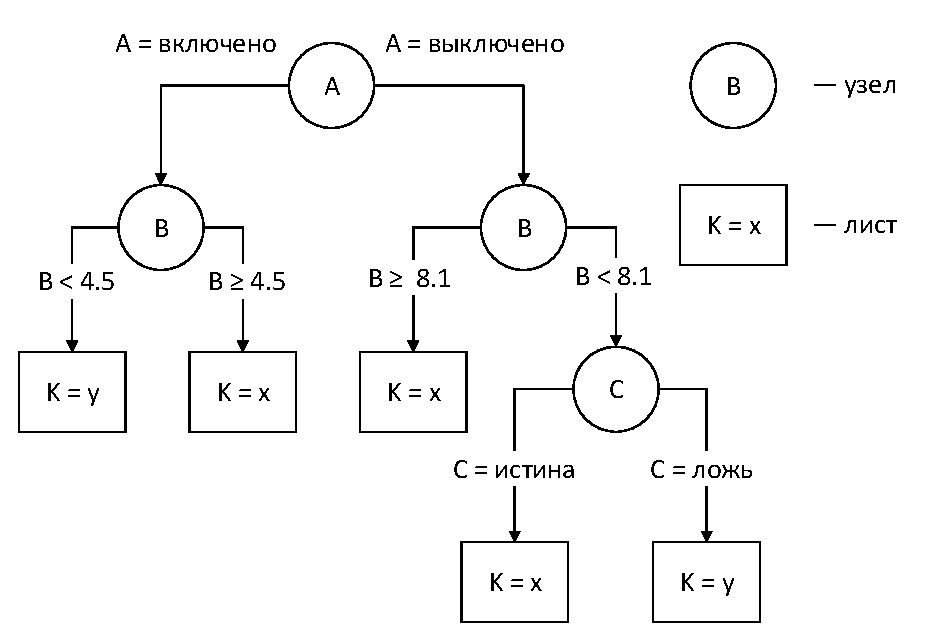
\includegraphics[width=0.7\textwidth, keepaspectratio]{decision_tree}
\caption{Пример дерева решений} \label{fig:spec:DecisionTreeExample}
\end{figure}

Так как алгоритм C4.5 относится к машинному обучению с учителем, GritBot дополняет его механизмом автоматического определения классов на основе вычисления статистических свойств выборки.

В исследовании~\cite{MLInCyberTrust} GritBot показал крайне низкую эффективность, не найдя ни одной добавленной в выборку аномалии. Это связано со статистическим подходим к определению аномальности объекта (метод ищет корреляцию между параметрами объектов в выборке). 

К преимуществам можно отнести лёгкость интерпретации результатов человеком (из-за использования деревьев решений можно получить набор правил, по которым пример был признан аномальным).

Недостатки:
\begin{itemize}
	\item низкая эффективность при наличии в выборке объектов с большим числом аномальных параметров~\cite{MLInCyberTrust};
	\item данный метод загружает весь массив исходных данных в память~\cite{BaySchwabacherOrca}; таким образом, с его помощью невозможно обрабатывать сколь-либо большие выборки;
	\item нет численной оценки степени аномальности примера (метод сортирует аномалии по их статистической значимости)~\cite{MartinCompUnsupervisedDetectionMethods}.
\end{itemize}

\subsection{GMM (Gaussian Mixture Model)}
GMM, или модель гауссовых смесей, наследует идеи Байесовской вероятности в том смысле, что она может быть легко представлена в рамках парадигмы графического моделирования.

Пример графической модели, представляющей гауссову смесь, показана на рисунке~\ref{fig:spec:GmmRepresentation}. Здесь $q_k\in \{1,\dots,M\}$, $\theta = (\pi_1,\dots,\pi_M,\mu_1,\dots,\mu_M,\Sigma_1,\dots,\Sigma_M)$. Закрашенные узлы представляют наблюдаемые непрерывные переменные, $y_k$ для момента времени $k$. Незакрашенные узлы, $q_k$, представляют $M$ ненаблюдаемых дискретных переменных, условная вероятность которых может быть вычислена на основе наблюдаемых данных. Параметры, содержащие $\theta$, могут быть выражены как функция от этих условных вероятностей и от других похоже сформированных оценок для каждой из $M$ гауссовых смесей, включая весовые коэффициенты смесей ($pi_i$), математические ожидания ($mu_i$) и матрицы ковариации ($\Sigma_i$).

\begin{figure}[h]
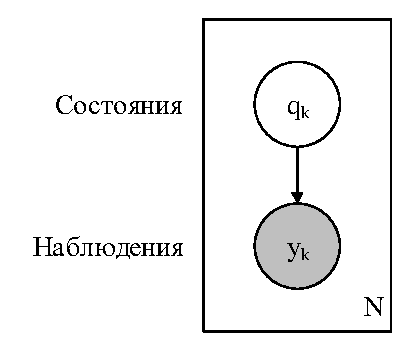
\includegraphics{gmm}
\caption{Графическое представление GMM без учителя}
\label{fig:spec:GmmRepresentation}
\end{figure}

Для использования данной модели требуется выполнение двух гипотез, представленных ниже.

\uline{Гипотеза о природе данных}: тестовые примеры появляются случайно и независимо, согласно вероятностному распределению, равному смеси распределений кластеров. Данное условие отображено в формуле~\eqref{eq:spec:GMM:Condition1}.

\begin{equation} \label{eq:spec:GMM:Condition1}
p(x) = \sum_{c\in C}^{} w_c p_c(x), \sum_{c\in C}^{} w_c = 1\text{,}
\end{equation}
\begin{description}
	\item[где $w_c$]~---~вероятность появления объектов из кластера $c$;
	\item[$p_c$]~---~плотность распределения кластера $c$.
\end{description}

\uline{Гипотеза о форме кластеров}: каждый кластер $c$ описывается $d$-мерной гауссовской плотностью с центром $\mu_c = \{\mu_{c1},\dots,\mu_{cd}\}$ и диагональной матрицей ковариации $\Sigma_c = diag(\sigma^2_{c1},\dots,\sigma^2_{cd})$ (т.е. по каждой координате своя дисперсия).

В этих предположениях для определения аномалий получается задача разделения смеси гауссовых распределений. Для этого обычно используется EM-алгоритм (expectation-maximization)~\cite{MartinCompUnsupervisedDetectionMethods}. Подробное описание данного алгоритма представлено в~\cite{KorolevEMAlgo}.

EM-алгоритм используется в математической статистике для нахождения оценок максимального правдоподобия параметров вероятностных моделей, в случае, когда модель зависит от некоторых скрытых переменных. Каждая итерация алгоритма состоит из двух шагов. На \textit{E-шаге (expectation)} вычисляется ожидаемое значение функции правдоподобия, при этом скрытые переменные рассматриваются как наблюдаемые. На \textit{M-шаге (maximization)} вычисляется оценка максимального правдоподобия, таким образом увеличивается ожидаемое правдоподобие, вычисляемое на E-шаге. Затем это значение используется для E-шага на следующей итерации. Алгоритм выполняется до сходимости.

Формальная постановка задачи разделения смеси гауссовых распределений выглядит следующим образом. Задана выбора $X^l$ случайных и независимых наблюдений из смеси $p(x)$, в которой описание $i$-го элемента есть вектор $x_i\in \mathbb{R}^n$. Принята модель, в которой каждая компонента смеси есть гауссиана с параметрами $\mu$ и $\Sigma$, и известно число компонентов смеси~---~$K$. Смесь показана в формуле~\eqref{eq:spec:GMM:Mixture}.

\begin{equation} \label{eq:spec:GMM:Mixture}
p(x) = \sum_{n=1}^{K} \pi_k N(x|\mu_k,\Sigma_k).
\end{equation}

Требуется оценить вектор параметров $\theta = (\pi_1,\dots,\pi_M,\mu_1,\dots,\mu_M,\Sigma_1,\dots,\Sigma_M)$, доставляющий максимум функции правдоподобия~\eqref{eq:spec:GMM:LikelihoodFunc}.

\begin{equation} \label{eq:spec:GMM:LikelihoodFunc}
\ln p(X|\pi,\mu,\Sigma) = \sum_{n=1}^{N} \ln \left\{\sum_{k=1}^{K} \pi_k N(x_n|\mu_k,\Sigma_k)\right\}
\end{equation}

Оптимальные параметры отыскиваются последовательно с помощью итерационного EM-алгоритма. Основная идея~–--~вводится вспомогательный вектор скрытых переменных. Это позволяет свести сложную оптимизационную задачу к последовательности итераций по пересчету коэффициентов (скрытых переменных по текущему приближению вектора параметров~---~E-шаг) и максимизации правдоподобия (с целью найти следующее приближение вектора~---~М-шаг).

В начале работы алгоритма задаются параметры начального приближения $\theta_0$. Далее итеративно выполняется следующая пара процедур:

\uline{E-шаг}: используя текущее значение вектора параметров $\theta$, вычисляется значение вектора скрытых переменных $\gamma$ по формуле~\eqref{eq:spec:GMM:HiddenVars}.

\begin{equation} \label{eq:spec:GMM:HiddenVars}
\gamma_{nk} = \frac{\pi_k N(x_n|\mu_k,\Sigma_k)}{\sum_{j=1}^{K} \pi_j N(x_n|\mu_j,\Sigma_j)}
\end{equation}

\uline{M-шаг}: переоценка вектора параметров по формулам~\eqref{eq:spec:GMM:newParams}, используя текущее значение вектора скрытых переменных.

\begin{subequations} \label{eq:spec:GMM:newParams}
\begin{equation} %\label{eq:spec:GMM:newMu}
\mu_k^{new} = \frac{1}{N_k} \sum_{n=1}^{N} \gamma_{nk} x_n \text{,}
\end{equation}
\begin{equation} %\label{eq:spec:GMM:newSigma}
\Sigma_k^{new} = \frac{1}{N_k} \sum_{n=1}^{N} \gamma_{nk} (x_n - \mu_k^{new})(x_n-\mu_k^{new})^T \text{,}
\end{equation}
\begin{equation} %\label{eq:spec:GMM:newPi}
\pi_k^{new} = \frac{N_k}{N} \text{,}
\end{equation}
\begin{equation} %\label{eq:spec:GMM:newN}
N_k = \sum_{n=1}^{N} \gamma_{nk} \text{,}
\end{equation}
\end{subequations}

Процедура останавливается после того, как норма разности векторов скрытых переменных на каждой итерации не будет превышать заданную константу~$\Delta$. Условие останова показно в~\eqref{eq:spec:GMM:StopCondition}.

\begin{equation} \label{eq:spec:GMM:StopCondition}
\delta_{max} = \max \left\{\delta_{max},|\gamma_{nk} - \gamma_{nk}^0|\right\} \leq\Delta
\end{equation}

Блок-схема алгоритма приведена в приложении~\ref{app:GMM:EMScheme}.

\subsection{Динамические байесовские сети (Dynamic Bayesian Network, DBN)}
Dynamic Bayesian Network, или динамическая байесовская сеть, является графической вероятностной моделью, представляющей собой множество переменных и их вероятностных зависимостей. Данный метод использует в своей работе формулу Байеса~\eqref{eq:spec:DBN:BayesTheorem}.

\begin{equation} \label{eq:spec:DBN:BayesTheorem}
P(A|B) = \frac{P(B|A) P(A)}{P(B)} \text{,}
\end{equation}
\begin{description}
	\item[где $P(A)$]~---~априорная вероятность гипотезы $A$;
	\item[$P(A|B)$]~---~вероятность гипотезы $A$ при наступлении события $B$ (апостериорная вероятность);
	\item[$P(B|A)$]~---~вероятность наступления события $B$ при истинности гипотезы $A$;
	\item[$P(B)$]~---~полная вероятность наступления события $B$.
\end{description}

Формула Байеса позволяет «переставить причину и следствие»: по известному факту события вычислить вероятность того, что оно было вызвано данной причиной. События, отражающие действие «причин», в данном случае называют \textit{гипотезами}, так как они~---~предполагаемые события, повлекшие данное. Безусловную вероятность справедливости гипотезы называют \textit{априорной} (насколько вероятна причина вообще), а условную~---~с учетом факта произошедшего события~---~\textit{апостериорной} (насколько вероятна причина оказалась с учетом данных о событии).

Формально байесовская сеть~---~это направленный ациклический граф, каждой вершине которого соответствует случайная переменная, а дуги графа кодируют отношения условной независимости между этими переменными. Вершины могут представлять переменные любых типов, быть взвешенными параметрами, скрытыми переменными или гипотезами. Если переменные байесовской сети являются дискретными случайными величинами, то такая сеть называется дискретной байесовской сетью. Байесовские сети, которые моделируют последовательности переменных, называют \textit{динамическими байесовскими сетями}~\cite{PearlDynamicBayesianNetworks}.

Если дуга выходит из вершины $A$ в вершину $B$, то $A$ называют родителем $B$, а $B$ называют потомком $A$. Если из вершины $A$ существует ориентированный путь в другую вершину $B$, то $B$ называется потомком $A$, а $A$ называется предком $B$. Множество вершин-родителей вершины $V_i$ обозначается как $parents(V_i) = PA_i$.

Направленный ациклический граф $G$ называется байесовской сетью для вероятностного распределения $P(v)$, заданного над множеством случайных переменных $V$, если каждой вершине графа поставлена в соответствие случайная переменная из $V$, а дуги в графе удовлетворяют условию (марковское условие): любая переменная $V_i$ из $V$ должна быть условно независима от всех вершин, не являющихся ее потомками, если заданы (получили означивание, обусловлены) все ее прямые родители $PA_i$ в графе $G$, то есть выполняется выражение~\eqref{eq:spec:DBN:BayesNetworkCondition}.

\begin{equation} \label{eq:spec:DBN:BayesNetworkCondition}
\forall V_i\in V: P(v_i|pa_i, s) = P(v_i|pa_i) \text{,}
\end{equation}
\begin{description}
	\item[где $v_i$]~---~значение $V_i$;
	\item[$S$]~---~множество всех вершин, не являющихся потомками $V_i$;
	\item[$s$]~---~конфигурация $S$;
	\item[$pa_i$]~---~конфигурация $PA_i$.
\end{description}

Тогда полное совместное распределение значений в вершинах можно удобно записать в виде декомпозиции (произведения) локальных распределений~\eqref{eq:spec:DBN:Distributions}.

\begin{equation} \label{eq:spec:DBN:Distributions}
P(V_1,\dots,V_n) = \prod_{i=1}^{n} P(V_i|parents(V_i))
\end{equation}

Если у вершины $V_i$ нет предков, то её локальное распределение вероятностей называют \textit{безусловным}, иначе \textit{условным}. Если вершина~---~случайная переменная получила означивание (например, в результате наблюдения), то такое означивание называют \textit{свидетельством}. Если значение переменной было установлено извне (а не наблюдалось), то такое означивание называется \textit{вмешательством} или \textit{интервенцией}~\cite{PearlDynamicBayesianNetworks}.

Условная независимость в байесовской сети представлена графическом свойством \textit{d-разделённости}. Пусть $X, Y, Z$~---~непересекающиеся подмножества вершин в ацикличном ориентированном графе $G$. Говорят, что множество вершин $Z$ d-разделяет $X$ и $Y$ тогда и только тогда, когда $Z$ блокирует все пути из любой вершины, принадлежащей $X$, в любую вершину, принадлежащую $Y$. Под путём понимается последовательность следующих друг за другом рёбер (любого направления) в графе.

В соответствии с теоремой о d-разделённости для ациклично ориентированного графа $G$ если вершины d-разделены, то они условно независимы; и если вершины условно-независимы во всех вероятностных распределениях, совместимых с графом G, то они d-разделены~\cite{PearlDynamicBayesianNetworks}.

Для динамических байесовских сетей существуют две возможных стратегии для поиска аномалий~\cite{DBNAnomalyDetection}: байесовский доверительный интервал (Bayesian Credible Interval, BCI) и максимальная апостериорная оценка измерений (maximum a posteriori measurement status, MAP-ms).

\subsubsection{Байесовский доверительный интервал (BCI)}
\label{subsubsec:spec:DBN:BCI}
Данная стратегия использует модель сети, представленную на рисунке~\ref{fig:spec:DBN:BCI}. Вектор $X$ представляет скрытые непрерывные переменные, вектор $M$~---~наблюдаемые непрерывные переменные. Нижние индексы обозначают моменты времени.

\begin{figure}[h]
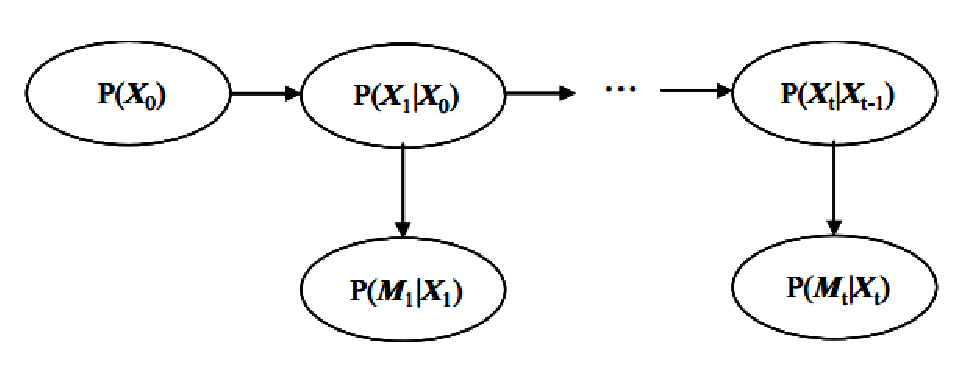
\includegraphics[width=0.7\textwidth]{dbn_bci}
\caption{Графическая модель сети для байесовского интервала правдоподобия (BCI)}
\label{fig:spec:DBN:BCI}
\end{figure}

Такая байесовская сеть отслеживает многомерные распределения линейных гауссовых переменных состояния и их наблюдаемые аналоги, которые измеряются с помощью датчиков. Скрытые переменные полагаются Марковскими процессами первого порядка, т.е. значение переменной в момент времени $t$ зависит только от состояния в момент времени $t-1$. Апостериорные вероятности скрытых и наблюдаемых переменных получаются с помощью фильтра Калмана, как только поступают новые измерения с датчиков. Данные вероятности используются для построения байесовского доверительного интервала $p\%$. Апостериорная вероятность $p$ отражает тот факт, что наблюдаемая переменная находится внутри интервала. Таким образом, любое измерение, попадающее за пределы доверительного интервала $p\%$, может быть классифицировано как аномалия~\cite{DBNAnomalyDetection}. Параметры сети (распределения вероятностей $P(X_0), P(X_t|X_{t-1}), P(M_t|X_t)$) могут быть получены из исходной выборки с помощью EM-алгоритма~\cite{KorolevEMAlgo}.

\subsubsection{Максимальная апостериорная оценка измерений (MAP-ms)}
В стратегии MAP-ms используется более сложная модель сети, показанная на рисунке~\ref{fig:spec:DBN:MAPms}. Векторы $X$ и $Z$ представляют непрерывные и дискретные скрытые переменные, а вектор $M$~---~наблюдаемые непрерывные переменные. Нижние индексы обозначают моменты времени.

\begin{figure}[h]
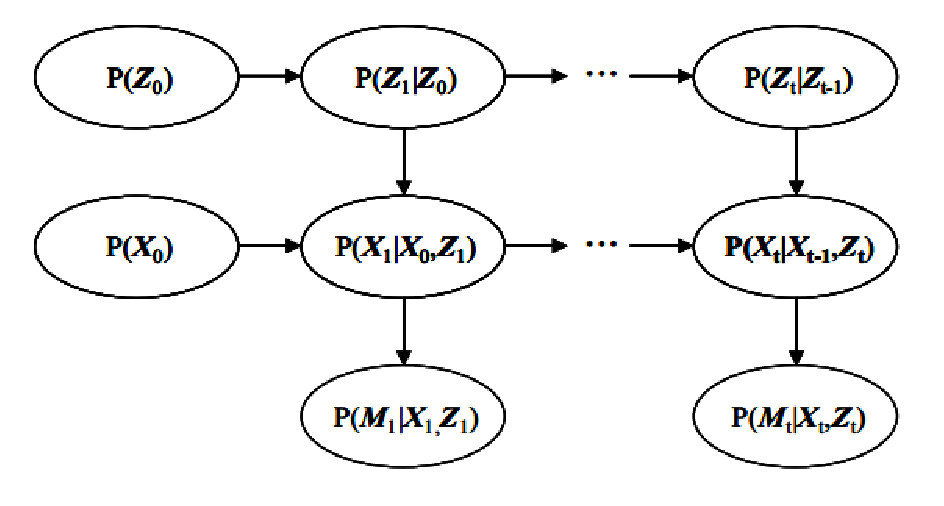
\includegraphics[width=0.7\textwidth]{dbn_mapms}
\caption{Графическая модель сети для максимального апостериорного статуса измерений (MAP-ms)}
\label{fig:spec:DBN:MAPms}
\end{figure}

Данная модель отслеживает многомерные многомерные распределения линейных гауссовых переменных состояния и их наблюдаемые аналоги, которые измеряются с помощью датчиков, как и вероятности скрытых дискретных переменных, показывающих статус каждого измерения (например, номинальный/аномальный). К примеру, если есть две измеряемых переменных состояния, то дискретная переменная статуса измерения будет иметь четыре возможных значения: (номинальный, номинальный), (аномальный, номинальный), (номинальный, аномальный) и (аномальный, аномальный). Апостериорные вероятности скрытых и наблюдаемых переменных получаются с помощью фильтра частиц Рао-Блэквелла, как только поступают новые измерения с датчиков. Максимальная апостериорная оценка измерения (например, наиболее вероятное значение, полученное из апостериорной вероятности) скрытой переменной состояния, показывающей статус измерения, может быть использована для классификации измерения как номинального или аномального. 

MAP-ms для работы требует, во-первых, параметры байесовской сети, описывающие изменение во времени линейных гауссовых переменных состояния для каждого значения дискретного статуса измерения, и, во-вторых, параметры, описывающие изменение во времени дискретных переменных. Кроме того, необходимо вручную задать вероятности для дискретных переменных ($P(Z_0), P(Z_t|Z_{t-1})$), опираясь на знание предметной области. Для случая, когда аномалий в исходной выборке нет, параметры сети совпадают с сетью для стратегии BCI, описанной в пункте~\ref{subsubsec:spec:DBN:BCI}. Если же одно или несколько измерений являются аномальными, параметры сети могут довольно сильно отличаться.~\cite{DBNAnomalyDetection}

Основные преимущества динамических байесовских сетей в применении к обнаружению аномалий:
\begin{itemize}
	\item способность работать в режиме реального времени~\cite{DBNAnomalyDetection};
	\item возможнсть графически представить модель системы.
\end{itemize}

Недостатки:
\begin{itemize}
	\item крайне высокая сложность метода;
	\item низкая эффективность на реальных данных~\cite{MartinCompUnsupervisedDetectionMethods}.
\end{itemize}

\subsection{One-Class SVM (Support Vector Machine)}
Метод опорных векторов~---~набор схожих алгоритмов обучения с учителем, использующихся для задач классификации и регрессионного анализа. One-Class SVM, или одноклассовый метод опорных векторов, представляет собой специальный вариант данного семейства для поиска аномалий, позволяющий использовать его в задачах обучения без учителя. В случае, если новое измерение принадлежит классу, оно считается номинальным (система работает в номинальном режиме); если же нет, то это измерение является аномалией. Особым свойством метода опорных векторов является непрерывное уменьшение эмпирической ошибки классификации и увеличение зазора, поэтому метод также известен как \textit{метод классификатора с максимальным зазором}.

Основная идея метода~---~перевод исходных векторов из низкой размерности, где они могут быть линейно неразделимы, в пространство более высокой размерности (вплоть до бесконечной) и поиск разделяющей гиперплоскости с максимальным зазором в этом пространстве. Две параллельных гиперплоскости строятся по обеим сторонам гиперплоскости, разделяющей классы. Разделяющей гиперплоскостью будет гиперплоскость, максимизирующая расстояние до двух параллельных гиперплоскостей. Алгоритм работает в предположении, что чем больше разница или расстояние между этими параллельными гиперплоскостями, тем меньше будет средняя ошибка классификатора~\cite{LifshitsInternetAlgorithms}.

Формальное описание задачи для случая с одним классом выглядит следующим образом: дана выборка $\Omega = \left\{x_1,x_2,\dots,x_n\right\}, x_i\in {\mathbb{R}}^m$, где $x_i$~---~точка в $m$-мерном пространстве, а $y_i\in \left\{0,1\right\}$ определяет принадлежность точки классу. Строится разделяющая гиперплоскость, которая имеет вид~\eqref{eq:spec:SVM:Hyperplane}, и гиперплоскость, параллельная ей~\eqref{eq:spec:SVM:ParallelHyperplane}.

\begin{subequations}
\begin{equation} \label{eq:spec:SVM:Hyperplane}
w^T x + b = 0 \text{;}
\end{equation}
\begin{equation}\label{eq:spec:SVM:ParallelHyperplane}
w^T x + b = 1 \text{,}
\end{equation}
\end{subequations}
\begin{description}
	\item[где $w\in \mathbb{F}$]~---~перпендикуляр к разделяющей гиперплоскости;
	\item[$b\in \mathbb{R}$]~---~расстояние по модулю от гиперплоскости до начала координат.
\end{description}

Если обучающая выборка линейно разделима, то возможно выбрать гиперплоскости таким образом, чтобы между ними не лежала ни одна точка обучающей выборки, и затем максимизировать расстояние между гиперплоскостями. Ширину полосы между ними легко найти из соображений геометрии, она равна $\frac{1}{\left\|w\right\|}$~\cite{VorontsovMachineLearning}, таким образом, задача сводится к минимизации $\left\|w\right\|$. Чтобы уберечь классифиактор от переполнения зашумлёнными данными, вводятся ошибки $\xi_i$, позволяющие некоторым точкам лежать внутри зазора, и константа $C > 0$, определяющая соотношение между максимизацией зазора и количеством точек внутри него (и, соответственно, ошибкой обучения). Целевая функция с учётом этих условий имеет вид~\eqref{eq:spec:SVM:ObjFunction}~\cite{RoemerIntroToOneClassSVM}.

\begin{equation} \label{eq:spec:SVM:ObjFunction}
\begin{aligned}
&\min_{w,b,\xi_i} \frac{{\left\|w\right\|}^2}{2} + C \sum_{i=1}^{n} \xi_i \text{,} \\
&y_i(w^T \phi(x_i) + b) \geq 1 - \xi_i &\text{ для всех } i = 1,\dots,n \text{,} \\
&\xi_i \geq 0 &\text{ для всех } i = 1,\dots,n \text{.}
\end{aligned}
\end{equation}

Оригинальная версия метода опорных вектров относится к семейству алгоритмов линейной классификации, что не подходит для задачи поиска аномалий в реальных многомерных данных. Существует способ создания нелинейного классификатора, в в основе которого лежит переход от скалярных произведений к произвольным ядрам, так называемый kernel trick, позволяющий строить нелинейные разделители. Результирующий алгоритм крайне похож на алгоритм линейной классификации, с той лишь разницей, что каждое скалярное произведение в приведённых выше формулах заменяется нелинейной функцией ядра (скалярным произведением в пространстве с большей размерностью). В этом пространстве уже может существовать оптимальная разделяющая гиперплоскость. Так как размерность получаемого пространства может быть больше размерности исходного, то преобразование, сопоставляющее скалярные произведения, будет нелинейным, а значит функция, соответствующая в исходном пространстве оптимальной разделяющей гиперплоскости, будет также нелинейной~\cite{LifshitsInternetAlgorithms}. Общий вид ядра показан в формуле~\eqref{eq:spec:SVM:KernelBasic}.

\begin{equation} \label{eq:spec:SVM:KernelBasic}
K(x,x_i) = \phi(x)^T\phi(x_i)
\end{equation}

Наиболее распространённые ядра~\cite{LifshitsInternetAlgorithms}: полиномиальное однородное~\eqref{eq:spec:SVM:Kernel:PolyHomogen}, полиномиальное неоднородное~\eqref{eq:spec:SVM:Kernel:PolyNoHomogen}, радиальная базисная функция~\eqref{eq:spec:SVM:Kernel:Basis}, радиальная базисная функция Гаусса~\eqref{eq:spec:SVM:Kernel:Gauss}.

\begin{subequations}
\begin{equation} \label{eq:spec:SVM:Kernel:PolyHomogen}
K(x,x_i) = (x \cdot x_i)^d \text{;}
\end{equation}
\begin{equation} \label{eq:spec:SVM:Kernel:PolyNoHomogen}
K(x,x_i) = (x \cdot x_i + 1)^d \text{;}
\end{equation}
\begin{equation} \label{eq:spec:SVM:Kernel:Basis}
K(x,x_i) = \exp (-\gamma{\left\|x - x_i\right\|}^2), \gamma > 0 \text{;}
\end{equation}
\begin{equation} \label{eq:spec:SVM:Kernel:Gauss}
K(x,x_i) = \exp (-\frac{{\left\|x - x_i\right\|}^2}{2\sigma^2}) \text{.}
\end{equation}
\end{subequations}

Преимущества метода:
\begin{itemize}
	\item метод сводится к решению задачи квадратичного программирования, которая всегда имеет единственное решение;
	\item даёт численную оценку аномальности (расстояние от точки до гиперплоскости)~\cite{MartinCompUnsupervisedDetectionMethods}.
\end{itemize}

Недостатки:
\begin{itemize}
	\item метод неустойчив по отношению к шуму в исходных данных. Если обучающая выборка содержит шумовые выбросы, они будут существенным образом учтены при построении разделяющей гиперплоскости;
	\item необходимо вручную подбирать функцию ядра, исходя из знаний о предметной области и природе исходных данных;
	\item в общем случае, когда линейная разделимость не гарантируется, приходится подбирать управляющий параметр алгоритма $C$~\cite{VorontsovMachineLearning};
	\item в случае значительных изменений в режиме работы системы не способен обнаруживать аномалии~\cite{MartinCompUnsupervisedDetectionMethods}.
\end{itemize}

\subsection{Inductive Monitoring System (IMS)}
\label{subsec:spec:IMS}
IMS автоматически строит базу знаний для последующего мониторинга состояния системы на основе номинальных данных, собранных непосредственно во время работы системы либо её симуляций. IMS использует машинное обучение и методы интеллектуального анализа данных для описания типичного для системы поведения путём извлечения из исходных данных основных классов. В частности, IMS использует кластеризацию для группировки постоянно встречающихся последовательностей в обучающей выборке. Кластеризация~---~семейство алгоритмов, относящееся к обучению без учителя, упорядочивающих объекты в сравнительно однородные группы (\textit{кластеры}). Идея метода IMS проистекает из двух алгоритмов кластеризации: алгоритма K-средних (K-means)~\cite{BradleyKMeans} и DBSCAN~\cite{EsterDensityBasedClustering} (кластеризация на основе плотности групп точек). Метод разработан Дэвидом Иверсоном (NASA Ames Research Center) и описан им в~\cite{IversonISHM}.

Базовой структурой данных для этого метода является вектор параметров системы. Пример подобного вектора приведён в таблице~\ref{tab:spec:IMS:SampleVector}. Каждый вектор содержит упорядоченный набор параметров, полученный системой мониторинга в процессе сбора телеметрии. Он также может содержать производные от измерений параметры. Векторы параметров системы представляют собой точки в $N$-мерном пространстве, которые IMS группирует в кластеры. Значения вектора могут быть получены подсистемой сбора данных как одновременно, либо быть собранными в вектор из нескольких измерений в течение некоторого периода времени. Размер и конкретные параметры вектора определяются вручную в соответствии с поставленной задачей мониторинга.

\begin{table}[h]
\caption{Пример вектора данных}
\label{tab:spec:IMS:SampleVector}

\begin{tabular}{|C{55pt}|C{50pt}|C{55pt}|C{50pt}|C{75pt}|C{75pt}|}
\hline
Давление A & Позиция клапана 1 & Давление B & Позиция клапана 2 & Температура 1 & Температура 2 \\
\hline
2857.2 & 86.4\% & 1218.4 & 96.2\% & 49.8 & 37.6 \\
\hline
\end{tabular}
\end{table}

IMS обрабатывает обучающую выборку, форматируя исходные данные в соответствии с заданной структурой вектора параметров, и строит базу знаний из кластеров. Пример подобного кластера приведён в таблице~\ref{tab:spec:IMS:SampleCluster}. Каждый кластер определяет диапазон допустимых значений всех переменных для входного вектора данных. Вектор верхней границы и вектор нижней границы в кластере могут быть представлены, как углы минимального ограничивающего гиперкуба в $N$-мерном пространстве. Точки, попадающие внутрь этого гиперкуба либо в его окрестность, классифицируются алгоритмом как относящиеся к номинальному режиму работы системы, так как гиперкуб определяется исходя из номинальных данных. Данный подход схож с интервальной диагностикой, когда строится математическая модель системы, и определяются допустимые диапазоны изменения каждой переменной, но не требует знаний о характере и устройстве системы.

\begin{table}[h]
\caption{Пример кластера}
\label{tab:spec:IMS:SampleCluster}

\begin{tabular}{|C{55pt}|C{55pt}|C{50pt}|C{55pt}|C{50pt}|C{75pt}|C{75pt}|}
\cline{2-7}
\multicolumn{1}{c|}{} & Давление A & Позиция клапана 1 & Давление B & Позиция клапана 2 & Температура 1 & Температура 2 \\
\hline
Верхняя граница & 2857.2 & 86.4\% & 1218.4 & 96.2\% & 49.8 & 37.6 \\
\hline
Нижная граница & 2857.2 & 86.4\% & 1218.4 & 96.2\%  & 49.8 & 37.6 \\
\hline
\end{tabular}
\end{table}

IMS начинает процесс обучения с пустой базы кластеров. Метод считывает элементы обучающей выборки и формирует из них в векторы. Первый вектор добавляется в базу, как исходный кластер. Каждый последующий вектор сравнивается с содержимым базы кластеров с тем, чтобы найти ближайший к этому вектору кластер. Для определения расстояния между вектором и кластером могут быть использованы различные метрики, например, Евклидово расстояние. Для того, чтобы найти расстояние от вектора до кластера, необходимо выбрать точку в кластере, до которой оно будет измерено. Одним из вариантов, основанным на алгоритме К-средних~\cite{BradleyKMeans}, является выбор центроида кластера, который рассчитывается как среднее между нижней и верхней границами. Для каждого нового вектора из обучающей выборки IMS находит в базе ближайший к нему кластер. Далее определяется, попадает ли вектор внутрь ограничивающего гиперкуба данного кластера или в его окрестность. Как и в кластеризации на основе плотности точек~\cite{EsterDensityBasedClustering}, вводится пороговое значение $\varepsilon$, заданное пользователем, которое определяет максимальное допустимое расстояние между вектором и кластером. На основе этого расстояния алгоритм определяет, стоит ли добавлять вектор в кластер. Если вектор достаточно близок (расстояние меньше или равно $\varepsilon$), границы кластера раздвигаются, чтобы вместить его. Если же расстояние превышает $\varepsilon$, создаётся новый кластер и добавляется в базу. Процесс обучения повторяется до тех пор, пока не будет обработана вся обучающая выборка. Малое значение $\varepsilon$ приводит к созданию небольших по размеру кластеров, что обеспечивает более точный контроль, но значительно увеличивает размер базы знаний, делая невозможным мониторинг системы в реальном времени. Значение $\varepsilon$ может быть подобрано таким образом, чтобы обеспечить баланс между скоростью работы и точностью контроля.

Блок-схема процесса обучения приведена в приложении~\ref{app:IMS:TrainingScheme}.

Результатом обработки IMS обучающей выборки является модель системы в виде базы кластеров, характеризующая работу системы в номинальных режимах, отображённых в исходных данных. В дополнение к этому, каждый кластер определяет ограничения на значения каждого из параметров в векторе.

Для использования получившейся базы кластеров для мониторинга состояния системы IMS формирует векторы из приходящих данных и запрашивает базу на предмет ближайшего к каждому входному вектору кластера. Наиболее быстрый способ проверки требует, чтобы все векторы находились внутри по крайней мере одного из кластеров внутри базы (значения всех параметров должны находиться внутри диапазонов, определённых границами кластера). Такой способ устраняет необходимость вычисления расстояний. Более информативная техника мониторинга находит ближайший к входному вектору кластер и показывает пользователю расстояние между ними. Это даёт оператору представление, насколько поведение системы отклоняется от нормального, представленного в обучающей выборке. Метод может учитывать неполноту обучающей выборки и неточности измерений путём задания порогового значения $\varepsilon$.

Блок-схема процесса мониторинга приведена в приложении~\ref{app:IMS:MonitoringScheme}.

Преимущества метода:
\begin{itemize}
	\item не требует больших вычислительных ресурсов, способен работать в реальном времени;
	\item предоставляет оператору численную характеристику аномальности вектора измерений;
	\item не имеет ограничений на закон распределения входных данных;
	\item не требует никаких знаний о предметной области, природе системы, её внутреннем устройстве, характеристиках входных данных, что обеспечивает универсальность и возможность применения к широкому спектру технических систем.
\end{itemize}

Недостатки:
\begin{itemize}
	\item метод неустойчив по отношению к шуму и аномалиям в обучающей выборке; 
	\item вектор входных данных может содержать только непрерывные переменные;
	\item стандартный вариант метода рассчитывает расстояние до центра кластера, что снижает точность мониторинга.
\end{itemize}

\section{Разработка метода мониторинга состояния ЛА на основе методов интеллектуального анализа данных}

Все описанные выше методы имеют свои недостатки при их применении для контроля состояния сложных технических систем. Сравнение методов по критериям, указанным в разделе~\ref{sec:spec:ProblemDefinition}, приведено в таблице~\ref{tab:spec:MethodsComparison}.

\begin{table}[h]
\caption{Сравнение методов выявления аномалий без учителя}
\label{tab:spec:MethodsComparison}

\begin{tabular}{|C{210pt}|C{35pt}|C{45pt}|C{38pt}|C{35pt}|C{36pt}|C{35pt}|}
\hline
\backslashbox{Критерий}{Метод} & Orca & GritBot & GMM & DBN & SVM & IMS \\
\hline
Построение модели ОК без априорных данных о предметной области, его назначении, составе, конструкции & + & + & ± & + & − & + \\
\hline
Классификация аномалий & − & − & − & + & − & − \\
\hline
Численная характеристика аномалии & + & − & − & − & + & + \\
\hline
Обработка больших выборок за конечное время & ± & − & ± & + & + & + \\
\hline
Работа с дискретными параметрами & + & + & − & ± & − & − \\
\hline
Отсутствие ограничений на закон распределения входных данных & + & + & − & ± & + & + \\
\hline
Устойчивость к аномалиям в обучающей выборке & + & + & − & − & − & − \\
\hline
Устойчивость к отсутствию значений параметров во входных данных & + & + & − & − & − & + \\
\hline
Работа в режиме реального времени & − & − & + & + & + & + \\
\hline
\end{tabular}
\end{table}

По результатам сравнения наиболее подходящим является метод IMS, описанный в подразделе~\ref{subsec:spec:IMS}. Так как он не удовлетворяет всем требованиям, указанным в разделе~\ref{sec:spec:ProblemDefinition}, необходимо создать на его основе метод, устойчивый к аномалиям в обучающей выборке, обеспечивающий возможность классификации аномалий и работающий не только с непрерывными, но и с дискретными параметрами.

\subsection{Формальная постановка задачи мониторинга системы}
\label{subsec:spec:DDMS:FormalTask}
Введём следующие обозначения:
\begin{description}
	\item[$M$]~---~дискретно-непрерывное пространство, имеющее $p$ непрерывных и $q$ дискретных измерений;
	\item[$R=\left\{R_1,R_2,\dots,R_n\right\} \in M$]~---~множество режимов работы системы;
	\item[$T=\left\{x_1,x_2,\dots,x_m\right\} \in M$]~---~обучающая выборка;
	\item[$x=\left\{a_1,a_2,\dots,a_p,b_1,b_2,\dots,b_q\right\} \in M, a_i\in\mathbb{R}, b_i\in\mathbb{N}$]~---~элемент обучающей выборки;
	\item[$\theta=\left\{\tilde{a}_1,\tilde{a}_2,\dots,\tilde{a}_p,\tilde{b}_1,\tilde{b}_2,\dots,\tilde{b}_q\right\} \in M, \tilde{a}_i\in\mathbb{R}, \tilde{b}_i\in\mathbb{N}$]~---~входной вектор;
	\item[$\Omega=\left\{\omega_1,\omega_2,\dots,\omega_{p+q}\right\}$]~---~вектор весов.
\end{description}

Необходимо отметить, что некоторые значения в векторах могут отсутствовать.
%\subsubsection{Определения}

Даны $n$ обучающих выборок $T_1\in R_1, T_2\in R_2,\dots, T_n\in R_n$ различной длины, содержащие $m_i$ элементов каждая, где $i$~---~номер режима работы системы. Дан вектор $\Omega$, содержащий веса, соответствующие важности каждого параметра системы. Дан входной вектор $\theta$.

Необходимо определить, принадлежит ли $\theta$ к $R$; если $\theta \in R$, то определить, в каком именно подмножестве $R_i\in R$ находится $\theta$. Если же $\theta \notin R$, найти численную меру $\lambda \in \mathbb{R}_{\geq 0}$, показывающую отклонение $\theta$ от $R$.

\subsection{Описание метода}
Предложенный ниже метод относится к методам, основанным на измерении расстояний между точками (distance-based). Поэтому для работы метода необходимо определить взвешенную метрику $d(x,y,\Omega)$ на пространстве $M$. В качестве такой метрики может выступать комбинация Евклидова расстояния~\eqref{eq:spec:DDMS:EuclidDistance} для непрерывных и функции отличия~\eqref{eq:spec:DDMS:DiffDistance} для дискретных переменных. Подобная метрика, определённая на пространстве $M$, показана в формуле~\eqref{eq:spec:DDMS:Distance}. В случае отсутствия значения прибавляется только вес данного параметра.

\begin{subequations}
\begin{equation} \label{eq:spec:DDMS:EuclidDistance}
D_E(x,y) = \sqrt{\sum_{i=1}^{n} \left(x_i - y_i\right)^2}
\end{equation}
\begin{equation} \label{eq:spec:DDMS:DiffDistance}
D_{diff}(x,y) = 
\begin{cases} 
	0, & x=y \text{,} \\
	1, & x\neq y \\
\end{cases}
\end{equation}
\end{subequations}

\begin{equation} \label{eq:spec:DDMS:Distance}
d(x,y,\Omega) = \sqrt{\sum_{i=1}^{p} \left[\omega_i \left(a_i^{(x)} - a_i^{(y)}\right)^2\right]} + \sum_{j=1}^{q} 
\left[\begin{cases} 
	0, & b_j^{(x)}=b_j^{(y)} \text{,} \\
	\omega_{j+p}, & b_j^{(x)}\neq b_j^{(y)} \\
\end{cases}\right]
\end{equation}

Блок-схема процесса обучения метода представлена в приложении~\ref{app:DDMS:TrainingScheme}.

Обучение метода проходит в два этапа: подготовка данных и формирование базы режимов.

Пример единицы входных данных для метода представлен в таблице~\ref{tab:spec:DDMS:SampleVector}.

\begin{table}[h]
\caption{Пример единицы входных данных разрабатываемого метода}
\label{tab:spec:DDMS:SampleVector}

\begin{tabular}{|C{55pt}|C{70pt}|C{55pt}|C{70pt}|C{75pt}|C{75pt}|}
\hline
Давление A & Состояние клапана 1 & Давление B & Состояние клапана 2 & Температура 1 & Температура 2 \\
\hline
2857.2 & Закрыт & 1218.4 & Открыт & 49.8 & 37.6 \\
\hline
\end{tabular}
\end{table}

\subsubsection{Подготовка данных}
\label{subsubsec:spec:DDMS:Preparing}
Формат входных данных, показанный в таблице~\ref{tab:spec:DDMS:SampleVector}, может не соответствовать формату, описанному в подразделе~\ref{subsec:spec:DDMS:FormalTask}. Для этого необходимо сгруппировать параметры по своей природе (отдельно непрерывные и отдельно дискретные). Для каждого дискретного параметра составляется список возможных значений, в соответствие которым ставятся натуральные числа.

Так как элементы в векторах могут иметь различный масштаб, для корректного определения расстояния между двумя точками непрерывные значения векторов сначала необходимо нормализовать. Для этого может применяться как минимаксная нормализация~\eqref{eq:spec:DDMS:MinimaxNormalization}, так и нормализация с помощью стандартного отклонения~\eqref{eq:spec:DDMS:StandardNormalization}. Метод сохраняет характеристики, используемые при нормализации обучающих вбыорок (минимум, среднее значение и т.д.), для масштабирования входного вектора на стадии мониторинга.

\begin{subequations}
\begin{equation} \label{eq:spec:DDMS:MinimaxNormalization}
\hat{x} = \frac{x - \min(X)}{\max(X) - \min(X)}, x\in X
\end{equation}
\begin{equation} \label{eq:spec:DDMS:StandardNormalization}
\hat{x} = \frac{x - \bar{x}}{\sigma_x} \text{,}
\end{equation}
\end{subequations}
\begin{description}
	\item[где $\bar{x}$]~---~среднее значение;
	\item[$\sigma_x$]~---~стандартное отклонение.
\end{description}

Зачастую в обучающих выборках могут содержаться аномальные элементы (сбой в работе датчика, искажения в канале связи и т.д.). Для того, чтобы метод мог корректно обучаться, необходимо их исключить. Для этого на каждой выборке используется алгоритм Orca, описанный в подразделе~\ref{subsec:spec:Orca}. В качестве количества аномалий, которые необходимо найти, ему задаётся число элементов в выборке. С учётом этой особенности на выходе данный алгоритм выдаёт численную меру (степень) аномальности для каждого вектора. Далее применяется фильтр, который на основе этой численной меры для каждого вектора определяет, является ли вектор аномальным. Для этого могут использоваться как статистические (например, Гауссовый фильтр, считающий аномальными все векторы, численная мера для которых не укладывается в диапазон $[0, 3\sigma]$), так и пороговые фильтры (считающие аномальными векторы, численная мера которых выше определённой величины $\delta$). Выбранные фильтром аномалии удаляются из выборки.

Результатом данного этапа являются нормализованные выборки $\hat{T}_i\in \hat{T}$, $i\in \left[1,n\right]$, не содержащие аномалий. Пример элемента такой выборки представлен в таблице~\ref{tab:spec:DDMS:PreparedSampleVector}.

\begin{table}[h]
\caption{Пример подготовленной единицы входных данных разрабатываемого метода}
\label{tab:spec:DDMS:PreparedSampleVector}

\begin{tabular}{|C{40pt}|C{40pt}|C{40pt}|C{40pt}|C{30pt}|C{30pt}|}
\hline
$a_1$ & $a_2$ & $a_3$ & $a_4$ & $b_1$ & $b_2$ \\
\hline
0.91 & 0.38 & 0.85 & 0.64 & 0 & 1 \\
\hline
\end{tabular}
\end{table}

\subsubsection{Формирование базы режимов}
На данном этапе производится создание отдельной базы кластеров для каждого режима работы системы $R_i$, $i\in \left[1,n\right]$. Блок-схема процесса представлена в приложении~\ref{app:DDMS:ClusterDBScheme}.

Каждый кластер определяет диапазон допустимых значений для непрерывных переменных $\left(a_1,a_2,\dots,a_p\right)$ и список допустимых значений для каждой дискретной переменной из $\left(b_1,b_2,\dots,b_q\right)$. Пример такого кластера представлен в таблице~. Вектор верхней границы и вектор нижней границы в кластере могут быть представлены, как углы минимального ограничивающего прямоугольного параллелепипеда в $p$-мерном пространстве ($p$~---~число непрерывных переменных в векторе).

\begin{table}[h]
\caption{Пример кластера разрабатываемого метода}
\label{tab:spec:DDMS:SampleCluster}

\begin{tabular}{|C{75pt}|C{40pt}|C{40pt}|C{40pt}|C{40pt}|C{30pt}|C{30pt}|}
\cline{2-7}
\multicolumn{1}{c|}{} & $a_1$ & $a_2$ & $a_3$ & $a_4$ & $b_1$ & $b_2$ \\
\hline
Верхняя граница & 0.91 & 0.38 & 0.85 & 0.64 & -- & -- \\
\hline
Нижняя граница & 0.45 & 0.45 & 0.55 & 0.14 & -- & -- \\
\hline
Допустимые значения & -- & -- & -- & -- & 0, 1 & 1 \\
\hline
\end{tabular}
\end{table}

Метод последовательно обрабатывает все векторы из выборки $T_i\in R_i$. Процесс начинается с пустой базой кластеров. Первым вектором инициализируется начальный кластер (нижняя и верхняя граница этого кластера считаются равными вектору, в списки допустимых значений дискретных переменных добавляются значения дискретных переменных вектора). Каждый последующий вектор сравнивается со всеми кластерами в базе. Если вектор полностью находится в границах кластера, то метод переходит к следующему вектору в обучающей выборке. Если вектор не попал ни в один кластер, то измеряется расстояние $d_c(x,c,\Omega)$ между вектором и всеми кластерами в базе с целью нахождения наиболее близкого кластера. Вводится пороговое значние $\varepsilon$, заданное пользователем, которое определяет максимальное допустимое расстояние между вектором и кластером (размер окрестности кластера). Если $d_c(x,c,\Omega) \leq \varepsilon$, то вектор находится в окрестности кластера и может быть включён в него. При этом границы кластера расширяются, чтобы включить в себя вектор, а в списки допустимых значений дискретных переменных добавляются соответствующие значения элементов вектора. Если же $d_c(x,c,\Omega) > \varepsilon$, то формируется новый кластер, инициализирующийся этим вектором, и добавляется в базу. Процесс обучения повторяется до тех пор, пока не будет обработана вся обучающая выборка. Малое значение $\varepsilon$ приводит к созданию небольших по размеру кластеров, что обеспечивает более точный контроль, но значительно увеличивает размер базы знаний, делая невозможным мониторинг системы в реальном времени. Значение $\varepsilon$ может быть подобрано таким образом, чтобы обеспечить баланс между скоростью работы и точностью контроля.

Функция расстояния $d_c(x,c,\Omega)$ может быть определена различными способами, зависящими от точки в кластере, до которой измеряется расстояние. В отличие от метода IMS, описанного в подразделе\ref{subsec:spec:IMS}, использующего расстояние до центра кластера (рисунок~\ref{fig:spec:DDMS:KMeansDistance}), предлагается использовать расстояние до ближайшей точки кластера (рисунок~\ref{fig:spec:DDMS:NearestDistance}), обеспечивающее более точную оценку удалённости вектора от границ кластера.

\begin{figure}[h]
	\begin{subfigure}[b]{0.35\textwidth}
		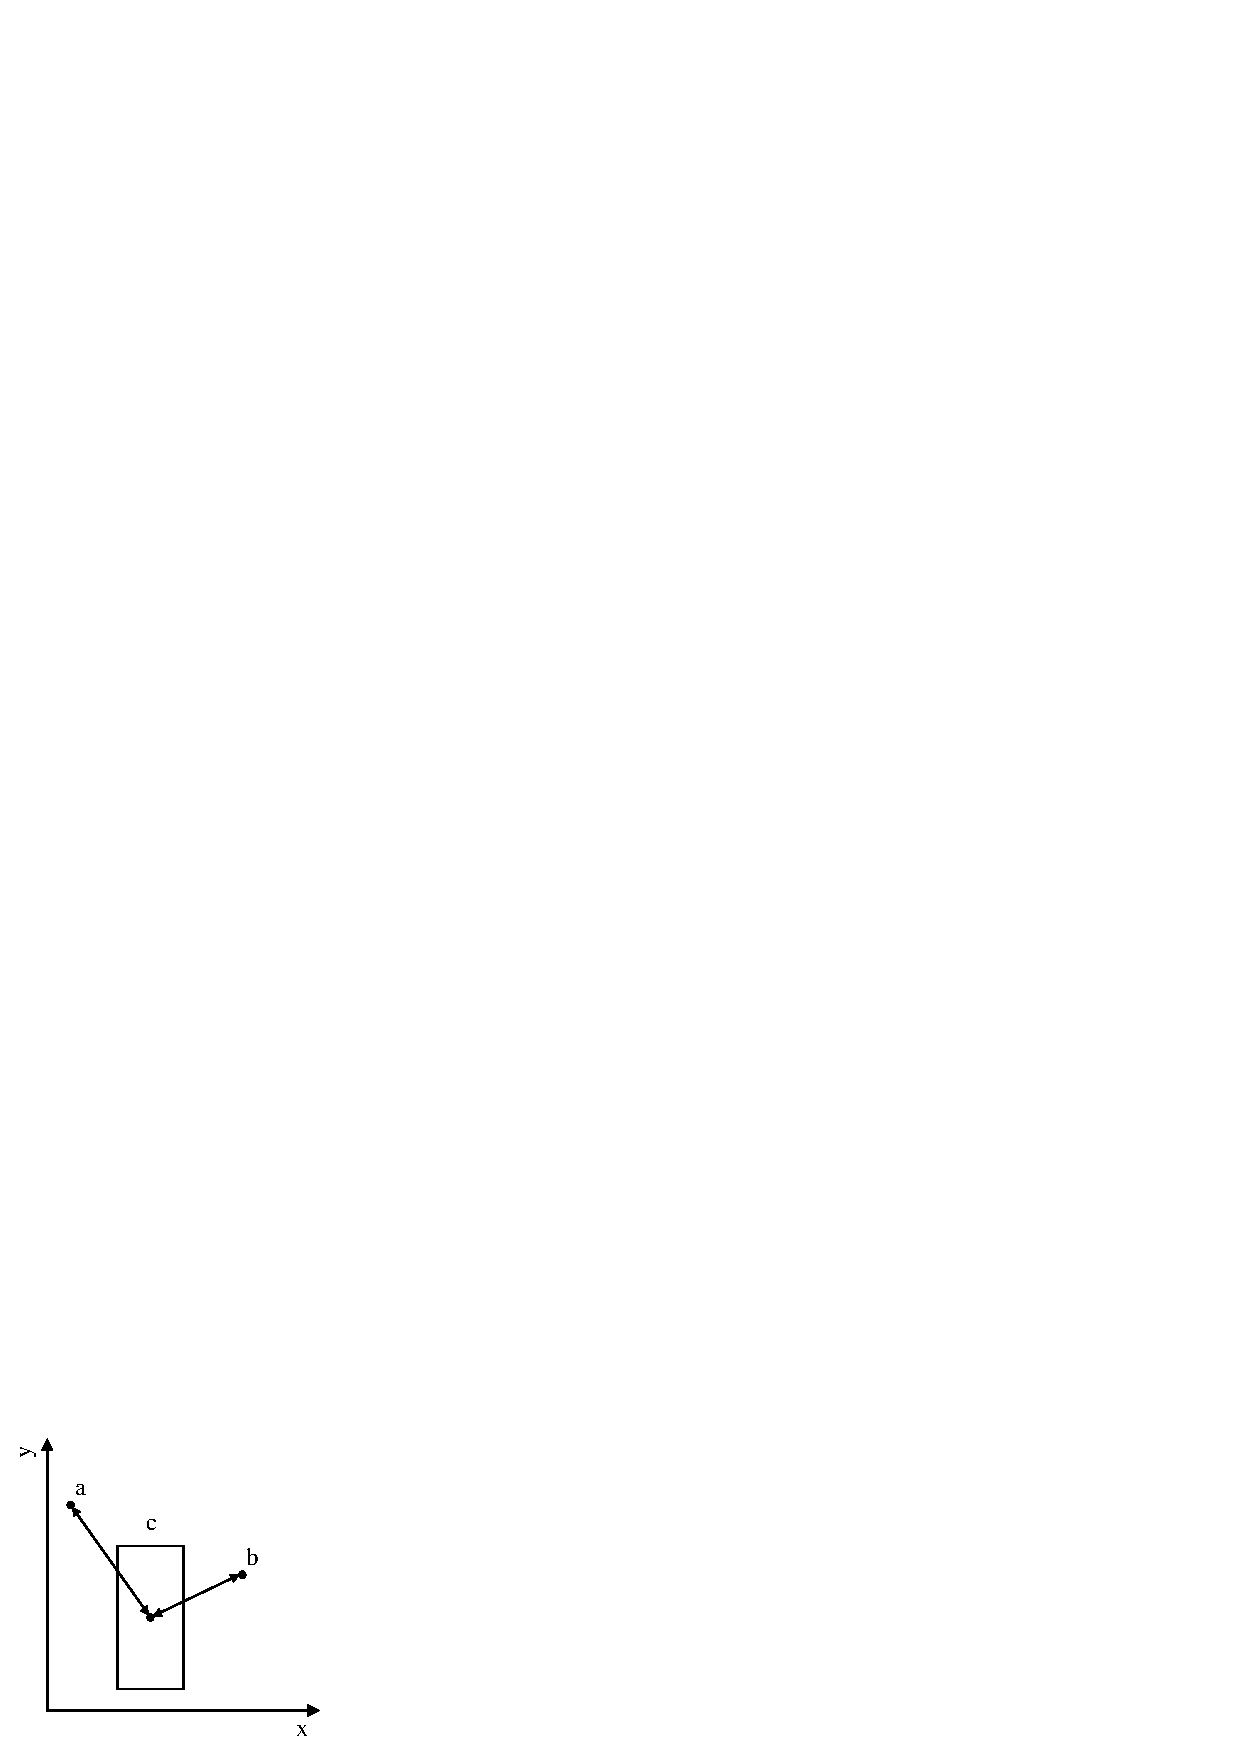
\includegraphics[width=\textwidth]{ddms_kmeans_distance}
		\caption{До центра кластера}
		\label{fig:spec:DDMS:KMeansDistance}
	\end{subfigure}
	\hspace{0.5cm}
	\begin{subfigure}[b]{0.35\textwidth}
		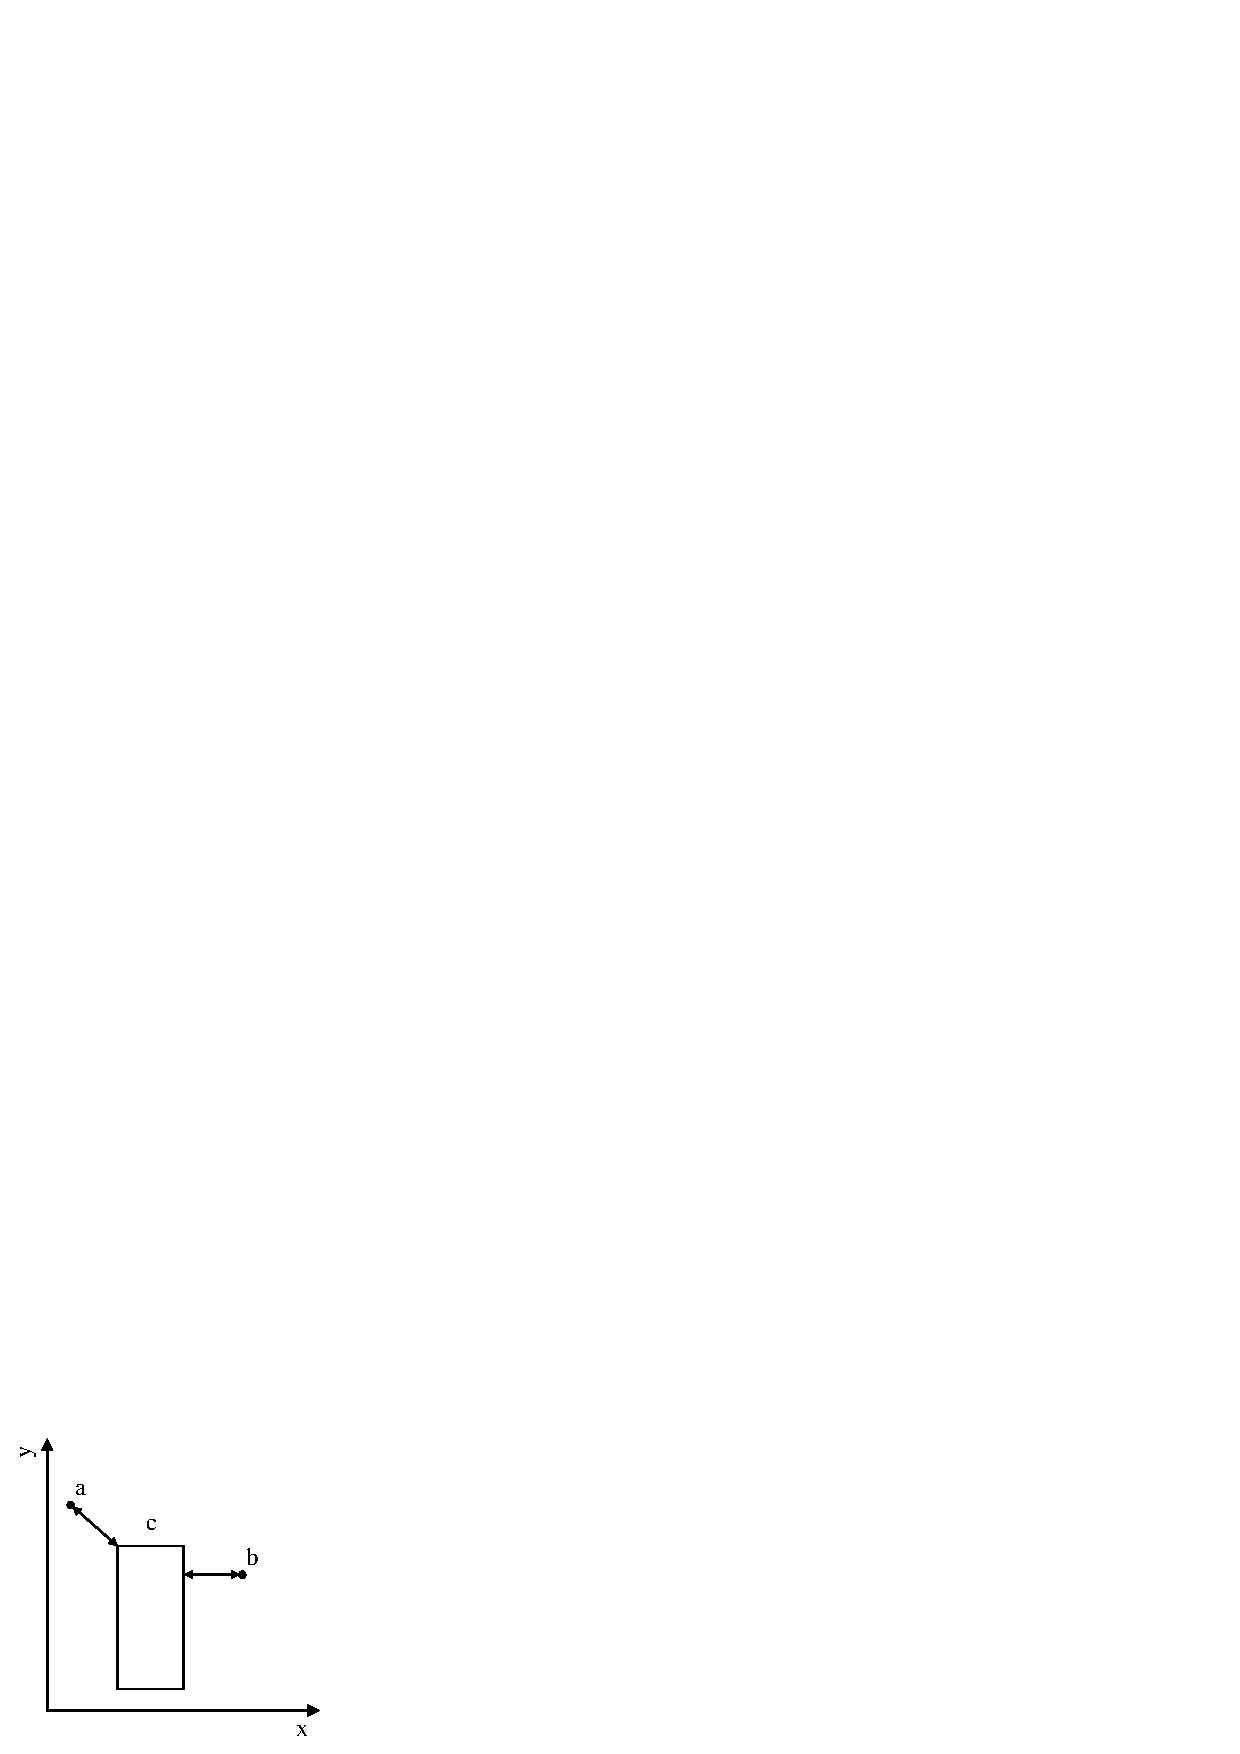
\includegraphics[width=\textwidth]{ddms_nearest_distance}
		\caption{До ближайшей точки кластера}
		\label{fig:spec:DDMS:NearestDistance}
	\end{subfigure}
	\caption{Виды расстояний от вектора до кластера}
\end{figure}

Результатом работы данного этапа является модель системы, состоящая из режимов, каждый из которых содержит базу кластеров. Структура модели показана на рисунке~\ref{fig:spec:DDMS:ModelStructure}.

\begin{figure}[h]
	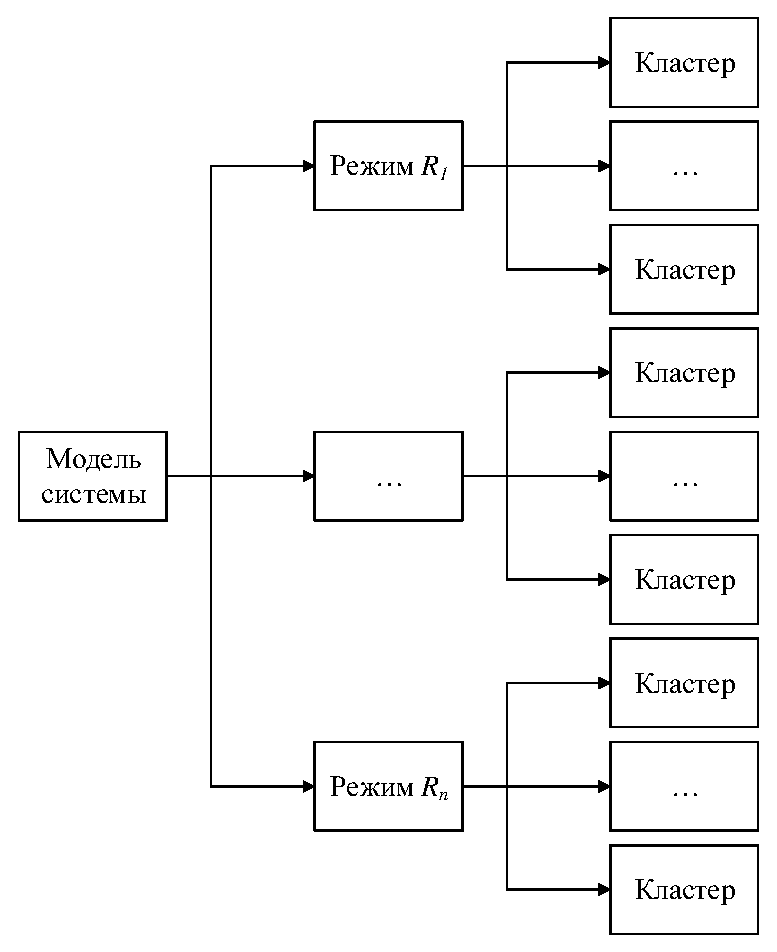
\includegraphics[height=0.45\textheight]{ddms_model_structure}
	\caption{Структура модели системы для разрабатываемого метода}
	\label{fig:spec:DDMS:ModelStructure}
\end{figure}

\subsubsection{Мониторинг состояния системы}
Для использования получившейся модели системы для мониторинга текущего состояния требуется получить из пришедшего вектора измерений входной вектор $\theta$ в формате, описанном в подразделе~\ref{subsec:spec:DDMS:FormalTask}, и нормализовать его. Для этого над вектором измерений производятся операции, описанные в пункте~\ref{subsubsec:spec:DDMS:Preparing}. Нормализация производится с использованием характеристик, сохранённых на аналогичном этапе при подготовке данных обучающих выборок.

Метод по очереди перебирает режимы и проверяет, находится ли входной вектор внутри одного из кластеров в базе режима. Если входной вектор попал внутрь кластера, то система работает в том режиме, к которому относится данный кластер. Иначе путём измерения расстояний $d_c(x,c,\Omega)$ от входного вектора до каждого кластера находится ближайший кластер. Если  $d_c(x,c,\Omega) \leq \varepsilon$, то вывод аналогичный с поправкой на то, что возможно отклонение от номинального поведения, поэтому метод даёт численную характеристику степени отклонения в виде расстояния $d_c(x,c,\Omega)$. В случае, когда $d_c(x,c,\Omega) > \varepsilon$ для всех кластеров во всех режимах, поведение системы считается аномальным; метод выводит ближайший режим и расстояние до него. Блок-схема данного процесса приведена в приложении~\ref{app:DDMS:MonitoringScheme}.

\section{Выбор программных средств реализации метода}

К языку программирования и программной платформе в данной работе предъявлялись следующие требования:
\begin{itemize}
	\item поддержка объектно-ориентированной парадигмы;
	\item удобство использования (скорость разработки);
	\item возможность повторного использования кода;
	\item быстродействие.
\end{itemize}

Рассмотрим подробнее каждое из требований.

\subsection{Предъявляемые требования}
\subsubsection{Поддержка объектно-ориентированной парадигмы}
Объектно-ориентированне программирование (ООП)~---~парадигма программирования, в которой основными концепциями являются понятия объектов и классов. В случае языков с прототипированием вместо классов используются объекты-прототипы. В центре ООП находится понятие объекта. Объект~---~это сущность, которой можно посылать сообщения и которая может на них реагировать, используя свои данные. Объект~---~это экземпляр класса. Данные объекта скрыты от остальной программы (инкапсулированы).
Наличие инкапсуляции достаточно для объектности языка программирования, но ещё не означает его объектной ориентированности~---~для этого требуется наличие наследования.
Но даже наличие инкапсуляции и наследования не делает язык программирования в полной мере объектным с точки зрения ООП. Основные преимущества ООП проявляются только в том случае, когда в языке программирования реализован полиморфизм; то есть возможность объектов с одинаковой спецификацией иметь различную реализацию.

Основные концепции и понятия ООП представлены ниже.

\uline{Абстрагирование}~---~это способ выделить набор значимых характеристик объекта, исключая из рассмотрения незначимые. Соответственно, абстракция — это набор всех таких характеристик.

\uline{Инкапсуляция}~---~это свойство системы, позволяющее объединить данные и методы, работающие с ними в классе, и скрыть детали реализации от пользователя.

\uline{Наследование}~---~это свойство системы, позволяющее описать новый класс на основе уже существующего с частично или полностью заимствующейся функциональностью. Класс, от которого производится наследование, называется базовым, родительским или суперклассом; новый класс~---~потомком, наследником или производным классом.

\uline{Полиморфизм}~---~это свойство системы использовать объекты с одинаковым интерфейсом без информации о типе и внутренней структуре объекта.

\uline{Класс}~---~описываемая на языке терминологии (пространства имён) исходного кода модель ещё не существующей сущности (объекта). Фактически он описывает устройство объекта, являясь своего рода чертежом. Говорят, что объект~---~это экземпляр класса. При этом в некоторых исполняющих системах класс также может представляться некоторым объектом при выполнении программы посредством динамической идентификации типа данных. Обычно классы разрабатывают таким образом, чтобы их объекты соответствовали объектам предметной области.

\uline{Объект}~---~сущность в адресном пространстве вычислительной системы, появляющаяся при создании экземпляра класса или копирования прототипа (например, после запуска результатов компиляции и связывания исходного кода на выполнение).

\uline{Прототип}~---~объект-образец, по образу и подобию которого создаются другие объекты. Объекты-копии могут сохранять связь с родительским объектом, автоматически наследуя изменения в прототипе; эта особенность определяется в рамках конкретного языка.~\cite{PaisonOOP}

Основными принципы объектно-ориентированного проектирования представлены ниже. Данный набор принципов принято обозначать аббревиатурой \textit{SOLID}.

\uline{Принцип единственной обязанности} (Single Responsibility Principle): каждый объект должен иметь одну обязанность и эта обязанность должна быть полностью инкапсулирована в класс. Все его сервисы должны быть направлены исключительно на обеспечение этой обязанности. Таким образом, класс или модуль должны иметь одну и только одну причину измениться.

\uline{Принцип открытости/закрытости} (Open/Closed Principle): программные сущности (классы, модули, функции и т.п.) должны быть открыты для расширения, но закрыты для изменения. Это означает, что такие сущности могут позволять менять свое поведение без изменения их исходного кода.

\uline{Принцип подстановки Барбары Лисков} (Liskov Substitution Principle): объекты в программе могут быть заменены их наследниками без изменения свойств программы. Функции, которые используют базовый тип, должны иметь возможность использовать подтипы (наследники) базового типа, не зная об этом.

\uline{Принцип разделения интерфейса} (Interface Segregation Principle): клиенты не должны зависеть от методов, которые они не используют. Интерфейсы, содержащие слишком много полей и методов, необходимо разделять на более маленькие и специфические, чтобы клиенты маленьких интерфейсов знали только о методах, которые необходимы им в работе. В итоге, при изменении метода интерфейса не должны меняться клиенты, которые этот метод не используют.

\uline{Принцип инверсии зависимостей} (Dependency Inversion Principle): зависимости внутри системы строятся на основе абстракций. Модули верхнего уровня не зависят от модулей нижнего уровня. Абстракции не должны зависеть от деталей. Детали должны зависеть от абстракций.~\cite{RMartinAgile}

Применение объектно-ориентированной парадигмы позволяет улучшить понимание исходного кода, упростить его дальнейшую поддержку, использование и усовершенствование, так как модули и классы в коде представляют собой проекции реальных объектов предметной области. В частности, в проектируемой системе такими объектами являются модель системы, режимы работы, кластеры, входные векторы и т.д. Поэтому требуется, чтобы язык программирования в полной мере поддерживал все концепции ООП.

\subsubsection{Удобство использования}
Под удобством использования подразумевается как логичность, приспособленность конструкций конкретного языка к поставленным задачам, так и удобство средств разработки (уже независимо от выбранного языка). Кроме того, следует учесть качество стандартной библиотеки и количество готовых компонентов (фреймворков, библиотек и т.п.), которые возможно использовать для решения типовых задач, программируя на данном языке. Удобство использования языка непосредственно влияет на время, затрачиваемое на написание программ на нём.

\subsubsection{Возможность повторного использования кода}
Повторное использование кода~---~методология проектирования компьютерных и других систем, заключающаяся в том, что система (компьютерная программа, программный модуль) частично либо полностью должна составляться из частей, написанных ранее компонентов и/или частей другой системы, и эти компоненты должны применяться более одного раза (если не в рамках одного проекта, то хотя бы разных). Повторное использование~---~основная методология, которая применяется для сокращения трудозатрат при разработке сложных систем.

Самый распространённый случай повторного использования кода~---~библиотеки программ. Библиотеки предоставляют общую достаточно универсальную функциональность, покрывающую избранную предметную область.

Данная система разрабатывается, как готовый программный продукт, однако должна быть возможность встраивания элементов системы (в частности, реализации метода диагностики аномалий) в другие программные продукты и системы. Также должна быть возможность доработки элементов системы другими специалистами, для которых специализированный или редко используемый язык может создать затруднения и увеличить затраты на использование модулей данной системы. Поэтому язык должен быть достаточно популярным в профессиональной среде и предоставлять средства для удобного создания модулей и отдельных библиотек.

\subsubsection{Быстродействие}
В зависимости от языка программирования быстродействие реализаций одного и того же алгоритма может значительно отличаться. Несмотря на то, что систему не предполагается использовать во встраиваемых ЭВМ, а ПЭВМ могут обеспечить мощности, более чем достаточные для подобной задачи, данный критерий всё равно представляется важным, так как система должна иметь возможность работать в режиме реального времени.

\subsection{Анализ языков программирования}
Наиболее распространёнными и набирающими популярность языками программирования, обеспечивающими полноценную поддержку ООП и позволяющими разрабатывать кроссплатформенные приложения для настольных ПЭВМ, являются следующие~\cite{TIOBELanguageIndex}:
\begin{itemize}
	\item C++;
	\item C\#;
	\item D;
	\item Java;
	\item Python;
	\item Ruby;
	\item Visual Basic .NET.
\end{itemize}

Рассмотрим каждый из них более подробно.

\subsubsection{C++}
С++~---~компилируемый статически типизированный язык программирования общего назначения. Поддерживает такие парадигмы программирования как процедурное программирование, объектно-ориентированное программирование, обобщённое программирование, обеспечивает модульность, раздельную компиляцию, обработку исключений, абстракцию данных, объявление типов (классов) объектов, виртуальные функции. Стандартная библиотека включает, в том числе, общеупотребительные контейнеры и алгоритмы.

Язык возник в начале 1980-х годов как разработка сотрудника Bell Labs Бьёрна Страуструпа. 

C++ широко используется для разработки программного обеспечения, являясь одним из самых популярных языков программирования~\cite{TIOBELanguageIndex}. Область его применения включает создание операционных систем, разнообразных прикладных программ, драйверов устройств, приложений для встраиваемых систем, высокопроизводительных серверов, а также развлекательных приложений (игр). Существует множество реализаций языка C++, как бесплатных, так и коммерческих и для различных платформ. Например, на платформе x86 это GCC, Visual C++, Intel C++ Compiler, Embarcadero (Borland) C++ Builder и другие. C++ оказал огромное влияние на другие языки программирования, в первую очередь на Java и C\#.

Преимущества:
\begin{itemize}
	\item достаточно высокая производительность. Язык спроектирован так, чтобы дать программисту максимальный контроль над всеми аспектами структуры и порядка исполнения программы. Имеется возможность работы с памятью на низком уровне.
	\item мультипарадигменность языка и широчайший спектр возможностей;
	\item огромное количество готовых библиотек и расширений.
\end{itemize}

Недостатки:
\begin{itemize}
	\item плохо продуманный синтаксис;
	\item унаследованные от языка Си низкоуровневые свойства существенно тормозят и затрудняют прикладную разработку;
	\item язык содержит опасные возможности, существенно снижающие качество и надёжность программ сразу по всем показателям.~\cite{WikiCpp}
\end{itemize}

\subsubsection{C\#}
C\#~---~мультипарадигменный язык программирования. Разработан в 1998—2001 годах группой инженеров под руководством Андерса Хейлсберга в компании Microsoft как язык разработки приложений для платформы Microsoft .NET Framework и впоследствии был стандартизирован как ECMA-334 и ISO/IEC 23270.

C\# относится к семье языков с C-подобным синтаксисом. Язык имеет поддержку статической и динамической типизации, поддерживает полиморфизм, перегрузку операторов (в том числе операторов явного и неявного приведения типа), делегаты, атрибуты, события, свойства, обобщённые типы и методы, итераторы, анонимные функции с поддержкой замыканий, LINQ, исключения, комментарии в формате XML.

Переняв многое от своих предшественников~---~языков C++, Pascal, Модула, Smalltalk и в особенности Java~---~С\#, опираясь на практику их использования, исключает некоторые модели, зарекомендовавшие себя как проблематичные при разработке программных систем, например, C\#, в отличие от C++, не поддерживает множественное наследование классов (между тем допускается множественное наследование интерфейсов).

Код на языке C\# транслируется в код на промежуточном языке MSIL (Microsoft Intermediate Language), который исполняется в виртуальной машине. Существует несколько реализаций для разных платформ. Хотя он и предназначен для генерации кода, исполняемого в среде .NET, сам по себе он не является частью .NET. Однако поскольку язык C\# предназначен для применения на платформе .NET, то разработчику, важно иметь представление о .NET Framework, если он хочет эффективно разрабатывать приложения на С\#. 

Центральной частью каркаса .NET является его Общеязыковая исполняющая среда – Common Language Runtime (CLR), или .NET runtime. Код, исполняемый под управлением CLR, часто называют управляемым кодом. Однако перед тем как код сможет исполниться CLR, любой исходный текст (на C\# или другом языке) должен быть скомпилирован. Компиляция в .NET состоит из двух шагов: 
\begin{itemize}
	\item компиляция исходного кода в IL; 
	\item компиляция IL в специфический для платформы код с помощью CLR.
\end{itemize}
 
Этот двухшаговый процесс компиляции очень важен, потому что наличие IL (управляемого кода)~---~это ключ ко многим преимуществам .NET.

К преимуществам .NET следует отнести наличие промежуточного языка Microsoft (MSIL).  MSIL разделяет с псевдокодом Java идею низкоуровневого языка с простым синтаксисом (базирующегося на числовых кодах вместо текста), который может быть очень быстро транслирован в родной машинный код. Наличие этого кода с четко определенным универсальным синтаксисом дает ряд существенных преимуществ. 
Это значит, что файл, содержащий инструкции псевдокода, может быть размещен на любой платформе; во время исполнения финальная стадия компиляции может быть легко осуществлена, что позволит выполнить код на конкретной платформе. Другими словами, компилируя в IL, вы получаете платформенную независимость .NET. 

Другим преимуществом подхода является повышение производительности. IL всегда компилируется оперативно (Just-In-Time, или JIT-компиляция). Вместо компиляции всего приложения за один проход (что может привести к задержкам при запуске), JIT-компилятор просто компилирует каждую порцию кода при ее вызове (just-in-time~---~оперативно). Если промежуточный код однажды скомпилирован, то результирующий машинный исполняемый код сохраняется до момента завершения работы приложения, поэтому его перекомпиляция при повторных вызовах не требуется.
 
Компания Microsoft заявляет, что такой процесс более эффективен, чем компиляция всего приложения при запуске, поскольку высока вероятность того, что большие куски кода приложения на самом деле не будут выполняться при каждом запуске. При использовании JIT-компилятора такой код никогда не будет скомпилирован. Это объясняет, почему можно рассчитывать на то, что выполнение родного управляемого кода IL будет почти настолько же быстрым, как и выполнение родного машинного кода. Финальная стадия компиляции проходит во время выполнения, JIT-компилятор на этот момент уже знает, на каком типе процессора будет запущена программа. Это значит, что он может оптимизировать финальный исполняемый код, используя инструкции конкретного машинного кода, предназначенные для конкретного процессора.

Преимущества:
\begin{itemize}
	\item мультипарадигменность;
	\item удобный и понятный синтаксис, поддерживающий огромное количество возможностей;
	\item наличие большой стандартной библиотеки;
	\item возможность интегрировать написанные на C\# модули в системы, написанные на других .NET-совместимых языках;
	\item наличие сборщика мусора;
	\item высокое быстродействие.
\end{itemize}

Недостатки: ограниченное использование во встраиваемых системах.~\cite{WikiCSharp}

\subsubsection{D}
D~---~компилируемый, статически и строго типизированный мултипарадигменный язык с Си-подобным синтаксисом, созданный Уолтером Брайтом из компании Digital Mars. Изначально был задуман как переосмысление языка C++, однако, несмотря на значительное влияние С++, не является его вариантом. В D были заново реализованы некоторые свойства C++, также язык испытал влияние концепций из других языков программирования, таких как Java, Python, Ruby, C\# и Eiffel. При создании языка D была сделана попытка соединить производительность компилируемых языков программирования с безопасностью и выразительностью динамических. Он является языком более высокого уровня, нежели C++. Выделение памяти в языке D полностью контролируется методикой «сборки мусора».

Преимущества:
\begin{itemize}
	\item высокая производительность;
	\item мультипарадигменность;
	\item наличие сборщика мусора;
	\item удобный и понятный синтаксис.
\end{itemize}

Недостатки:
\begin{itemize}
	\item язык только набирает популярность, поэтому число пользователей не так велико, как у других языков;
	\item непродуманная и имеющая ограниченный функционал стандартная библиотека.~\cite{WikiD}
\end{itemize}

\subsubsection{Java}
Java~---~объектно-ориентированный язык программирования, разработанный компанией Sun Microsystems (в последующем приобретённой компанией Oracle). Приложения Java обычно транслируется в специальный байт-код, поэтому они могут работать на любой виртуальной Java-машине (JVM) вне зависимости от компьютерной архитектуры. Дата официального выпуска~---~23 мая 1995 года.

Программы на Java транслируются в байт-код, выполняемый виртуальной машиной Java (JVM) — программой, обрабатывающей байтовый код и передающей инструкции оборудованию как интерпретатор.
Дюк, талисман Java

Достоинством подобного способа выполнения программ является полная независимость байт-кода от операционной системы и оборудования, что позволяет выполнять Java-приложения на любом устройстве, для которого существует соответствующая виртуальная машина. Другой важной особенностью технологии Java является гибкая система безопасности благодаря тому, что исполнение программы полностью контролируется виртуальной машиной. Любые операции, которые превышают установленные полномочия программы (например, попытка несанкционированного доступа к данным или соединения с другим компьютером) вызывают немедленное прерывание.

Разработка приложений с использованием языка Java производится быстрее, чем на С++, так как Java избавлена от низкоуровневых проблем (таких, как, например, выделение и освобождение памяти вручную).

Преимущества:
\begin{itemize}
	\item высокая распространённость языка;
	\item большое количество готовых библиотек и компонентов;
	\item богатая встроенная библиотека.
\end{itemize}

Недостатки:
\begin{itemize}
	\item низкая производительность, связанная с реализацией виртуальной машины (JVM);
	\item ограниченные возможности языка.~\cite{WikiJava}
\end{itemize}

\subsubsection{Python}
Python~---~высокоуровневый язык программирования общего назначения, ориентированный на повышение производительности разработчика и читаемости кода. Синтаксис ядра Python минималистичен. Python поддерживает динамическую типизацию, то есть тип переменной определяется только во время исполнения. В то же время стандартная библиотека включает большой объём полезных функций. Разработка языка Python была начата в конце 1980-х годов сотрудником голландского института CWI Гвидо ван Россумом.

Python поддерживает несколько парадигм программирования, в том числе структурное, объектно-ориентированное, функциональное, императивное и аспектно-ориентированное. Основные архитектурные черты — динамическая типизация, автоматическое управление памятью, полная интроспекция, механизм обработки исключений, поддержка многопоточных вычислений и удобные высокоуровневые структуры данных. Код в Питоне организовывается в функции и классы, которые могут объединяться в модули (они в свою очередь могут быть объединены в пакеты).

Эталонной реализацией Python является интерпретатор CPython, поддерживающий большинство активно используемых платформ. Есть реализации интерпретаторов для JVM (с возможностью компиляции), MSIL (с возможностью компиляции), LLVM и других.

Преимущества:
\begin{itemize}
	\item синтаксис поддерживает большое число функций;
	\item существуют реализации языка для многих популярных платформ и виртуальных машин;
	\item богатая встроенная библиотека.
\end{itemize}

Недостатки:
\begin{itemize}
	\item низкая производительность в интерпретируемых реализациях;
	\item отсутствие концепции будущего развития языка.~\cite{WikiPython}
\end{itemize}

\subsubsection{Ruby}
Ruby~---~динамический, рефлективный, интерпретируемый высокоуровневый язык программирования для быстрого и удобного объектно-ориентированного программирования. Язык обладает независимой от операционной системы реализацией многопоточности, строгой динамической типизацией, сборщиком мусора и многими другими возможностями. Ruby близок по особенностям синтаксиса к языкам Perl и Eiffel, по объектно-ориентированному подходу~---~к Smalltalk. Также некоторые черты языка взяты из Python, Lisp, Dylan и CLU. Создателем языка является Юкихиро Мацумото. Первая версия была опубликована в 1995 году.

Ruby~---~полностью объектно-ориентированный язык. В нём все данные являются объектами, в отличие от многих других языков, где существуют примитивные типы. Каждая функция~---~метод. Ruby является мультипарадигменным языком: он поддерживает процедурный стиль (определение функций и переменных вне классов), объектно-ориентированный (всё~---~объект), функциональный (анонимные функции, замыкания, возврат значения всеми инструкциями, возврат функцией последнего вычисленного значения). Он поддерживает отражение, метапрограммирование, информацию о типах переменных на стадии выполнения.

Для Ruby существуют несколько реализаций: официальный интерпретатор, написанный на Си, JRuby~---~реализация для Java, интерпретатор для платформы .NET IronRuby и др.

Преимущества:
\begin{itemize}
	\item существуют реализации языка для многих популярных платформ и виртуальных машин;
	\item язык имеет лаконичный синтаксис.
\end{itemize}

Недостатки:
\begin{itemize}
	\item низкая производительность в интерпретируемых реализациях;
	\item низкая популярность языка при создании технических систем.~\cite{WikiRuby}
\end{itemize}

\subsubsection{Visual Basic .NET}
Visual Basic .NET~---~объектно-ориентированный язык программирования, реализация языка Visual Basic для платформы .NET.

Преимущества:
\begin{itemize}
	\item простой синтаксис;
	\item возможность интеграции в любые системы на платформе .NET.
\end{itemize}

Недостатки:
\begin{itemize}
	\item ограниченность синтаксиса;
	\item концепция языка является устаревшей и не подвергается серьёзным изменениям.~\cite{WikiVBNet}
\end{itemize}

\subsection{Выбор языка программирования}
Проведя анализ вышеописанных языков программирования, можно заключить, что язык C\# является наиболее подходящим для разработки данной системы. Немаловажным обстоятельством является то, что именно этот язык является наиболее знакомым автору из всех рассмотренных, что служит дополнительным плюсом в пользу данного языка, так как на изучение всех особенностей другого языка может уйти большое количество времени. Зачастую именно грамотное использование всех особенностей языка и встроенной библиотеки и обуславливает написание качественного кода.

\section{Разработка программной реализации метода}
Программная реализация была разработана на языке программирование C\# 5.0 с использованием фреймворка .NET 4.5 в среде Microsoft Visual Studio 2013. Система разработана таким образом, чтобы обеспечить универсальность и лёгкость интеграции в другие смежные системы, позволить повторное использование отдельных модулей. Она имеет текстовый (консольный) интерфейс в соответствии с философией UNIX для возможности использования из других программных систем. Исходный код приведён в приложении~\ref{app:SourceCode}.

\subsection{Архитектура системы}
Архитектура системы проектировалась с учётом возможного расширения и дополнения функционала. Система имеет модульную структуру. Основные функциональные модули:
\begin{itemize}
	\item Thesis.DDMS~---~реализация разработанного метода;
	\item Thesis.Orca~---~реализация алгоритма Orca, описанного в пункте~\ref{subsec:spec:Orca};
	\item Thesis.DataCleansing~---~реализация фильтров, используемых для очищения обучающих выборок от аномалий;
	\item Thesis.Miscellaneous~---~содержит общие классы предметной области, абстракции и функционал, используемый в остальных модулях;
	\item Thesis.App~---~программное приложение (исполняемый файл), связывающее воедино остальные модули и предоставляющее интерфейс пользователя.
\end{itemize}

\subsubsection{Чтение и обработка входных данных}
Реализовано чтение из текстовых и бинарных файлов специального формата. Для обеспечения возможности добавления поддержки других источников и форматов данных представлены абстракции чтения и записи обучающих выборок и синтаксического анализа данных телеметрии.

UML-диаграмма классов, отвечающих за операции над данными, приведена в приложении~\ref{app:UML:Class:DataOperations}. Описание элементов представлено ниже.

\uline{FieldType}~---~тип параметра в векторах входных данных. Возможные значения: \textit{IgnoreFeature} (игнорировать данный параметр при чтении), \textit{Continuous} (непрерывный параметр), \textit{Discrete} (дискретный с фиксированным множеством значений), \textit{DiscreteDataDriven} (дискретный, возможные значения параметра получаются из входных данных).

\uline{Field}~---~класс параметра. Имеет имя, тип, весовой коэффициент, список возможных значений (для дискретных параметров).

\uline{Record}~---~вектор данных (запись). Содержит идентификатор, значения непрерывных и дискретных параметров.

\uline{IRecordParser<T>}~---~абстракция над конвертером, преобразующим единицу входных данных (строку, значения датчиков, подключенных к системе, и т.п.) в вектор (запись) типа \textit{Record}.

\uline{PlainTextParser}~---~реализация конвертера \textit{IRecordParser} для преобразования текстовой строки в вектор.

\uline{DataFormatException}~---~исключение, создающееся при ошибках в текстовых входных данных.

\uline{StringHelper}~---~класс с вспомогательными методами для обработки строк. Позволяет разбить строку на части, используя указанные символы-разделители.

\uline{IDataReader}~---~абстракция над чтением из источника данных. Предоставляет интерфейс для чтения векторов, сброса источника на начальную позицию, получения текущей позиции, описания параметров векторов и флага достижения конца данных.

\uline{IDataWriter}~---~абстракция над записью в источник данных. Предоставляет интерфейс для записи вектора и получения количества уже записанных векторов.

\uline{PlainTextReader}~---~реализация интерфейса \textit{IDataReader} для чтения описания параметров и обучающих выборок из текстовых файлов.

\uline{BinaryDataReader}~---~реализация интерфейса \textit{IDataReader} для чтения описания параметров и обучающих выборок из бинарных файлов специального формата.

\uline{BinaryDataWriter}~---~реализация интерфейса \textit{IDataWriter} для записи описания параметров и обучающих выборок в бинарные файлы специального формата.

\uline{BatchDataReader}~---~реализация интерфейса \textit{IDataReader} для чтения записей блоками по указанному количеству штук. Представляет собой реализацию паттерна декоратор~\cite{GangOfFourDesignPatterns} над объектом типа \textit{IDataReader}.

\uline{IScaling}~---~абстракция над методом нормализации данных. Предоставляет интерфейс для прямого и обратного масштабирования вектора или только его непрерывных параметров.

\uline{MinmaxScaling}~---~реализация интерфейса \textit{IScaling} для минимаксной нормализации по формуле~\eqref{eq:spec:DDMS:MinimaxNormalization}.

\uline{StandardScaling}~---~реализация интерфейса \textit{IScaling} для нормализации с помощью стандартного отклонения по формуле~\eqref{eq:spec:DDMS:StandardNormalization}.

\uline{ScaleDataReader}~---~реализация интерфейса \textit{IDataReader} для нормализации данных при чтении из источника. Представляет собой реализацию паттерна декоратор~\cite{GangOfFourDesignPatterns} над объектом типа \textit{IDataReader}.

\subsubsection{Поиск аномалий в обучающих выборках с помощью алгоритма Orca}
UML-диаграмма классов для поиска аномалий в обучающих выборках приведена в приложении~\ref{app:UML:Class:Orca}. Описание элементов представлено ниже.

\uline{OrcaAD}~---~класс, реализующий алгоритм Orca (см. подраздел~\ref{subsec:spec:Orca}).

\uline{Outlier}~---~структура данных, хранящая информацию об аномалии. Содержит идентификатор записи и значение степени аномальности.

\uline{BinaryShuffle}~---~реализует рандомизацию данных обучающей выборки (требуется для работы алгоритма Orca). Записывает рандомизированные данные в бинарный файл. Рандомизация происходит в $n$ итераций следующим образом: создаётся $m$ временных файлов, в которые случайным образом распределяются элементы обучающей выборки. Затем файлы объединяются в порядке, определяемом с помощью перетасовки Дональда Кнута~\cite{KnuthSeminumAlgo}.

\uline{DataHelper}~---~предоставляет удобный интерфейс для класса BinaryShuffle.

\uline{ScoreFunction}~---~описывает тип функции оценки степени аномальности для алгоритма Orca. Класс \uline{ScoreFunctions} содержит несколько вариантов таких функций.

\uline{BinaryHeap}~---~реализация структуры данных «двоичная куча»~\cite{AlgorithmsCormen}. Используется алгоритмом Orca для определения наиболее удалённых ближайших соседей.

\subsubsection{Очистка обучающих выборок от аномалий}
UML-диаграмма классов, используемых для очистки обучающих выборок от аномалий, приведена в приложении~\ref{app:UML:Class:DataCleansing}. Описание элементов представлено ниже.

\uline{IAnomaliesFilter}~---~абстракция над типом фильтра аномалий. Предоставляет интерфейс для метода \textit{Filter}, принимающего на вход коллекцию объектов типа \textit{Outlier} и возвращающего из неё только те элементы, которые прошли через фильтр (которые являются аномалиями).

\uline{DifferenceFilter}~---~разностный фильтр. Псевдокод алгоритма фильтрации показан в листинге~\ref{lst:spec:Filters:DiffPseudocode}.

\begin{algorithm}[hb!]
\caption{Псевдокод алгоритма фильтрации для разностного фильтра}
\label{lst:spec:Filters:DiffPseudocode}
\begin{algorithmic}[1]
\REQUIRE значения степени аномальности для записей в обучающей выборке, отсортированные по убыванию; $\Delta$, максимальная разность степеней аномальности для двух подряд идущих записей
\ENSURE аномальные записи
\IF{количество записей $< 2$}
	\RETURN $\varnothing$
\ENDIF
\FOR{$i$ от количества записей в выборке до $0$}
	\STATE $\delta \leftarrow$ разность значений степени аномальности ($i-1$)-й и $i$-й записей
	\IF{$\delta > \Delta$}
		\RETURN $i$ записей с самыми большими значениями степени аномальности
	\ENDIF
\ENDFOR
\RETURN $\varnothing$
\end{algorithmic}
\end{algorithm}

\uline{ThresholdFilter}~---~пороговый фильтр. Псевдокод алгоритма фильтрации показан в листинге~\ref{lst:spec:Filters:ThresholdPseudocode}.

\begin{algorithm}[hb!]
\caption{Псевдокод алгоритма фильтрации для порогового фильтра}
\label{lst:spec:Filters:ThresholdPseudocode}
\begin{algorithmic}[1]
\REQUIRE значения степени аномальности для записей в обучающей выборке, отсортированные по убыванию; $\rho$, максимальное значение степени аномальности
\ENSURE аномальные записи
\STATE $\mu \leftarrow$ минимальное значение степени аномальности для всех записей в обучающей выборке
\FORALL{записей в выборке}
	\STATE $x \leftarrow$ значение степени аномальности текущей записи
	\IF{$x - \mu > \rho$}
		\RETURN текущую запись
	\ENDIF
\ENDFOR
\end{algorithmic}
\end{algorithm}

\uline{GaussianFilter}~---~гауссовый фильтр. Псевдокод алгоритма фильтрации показан в листинге~\ref{lst:spec:Filters:GaussianPseudocode}.

\begin{algorithm}[h!]
\caption{Псевдокод алгоритма фильтрации для гауссового фильтра}
\label{lst:spec:Filters:GaussianPseudocode}
\begin{algorithmic}[1]
\REQUIRE значения степени аномальности для записей в обучающей выборке, отсортированные по убыванию
\ENSURE аномальные записи
\STATE $M \leftarrow$ мат. ожидание степени аномальности
\STATE $D \leftarrow$ дисперсия степени аномальности
\STATE $\sigma \leftarrow \sqrt{D}$
\FORALL{записей в выборке}
	\STATE $x \leftarrow$ значение степени аномальности текущей записи
	\IF{$x > M + 3\sigma$}
		\RETURN текущую запись
	\ENDIF
\ENDFOR
\end{algorithmic}
\end{algorithm}

\uline{ScaleDataReader}~---~реализация интерфейса \textit{IDataReader} для пропуска аномальных записей при чтении из источника. Если текущая запись является аномальной, то объект данного класса переходит к следующей записи. Представляет собой реализацию паттерна декоратор~\cite{GangOfFourDesignPatterns} над объектом типа \textit{IDataReader}.

\subsubsection{Построение модели ОК}
UML-диаграмма классов для построения модели ОК приведена в приложении~\ref{app:UML:Class:DDMS}. Описание элементов представлено ниже.

\uline{DistanceMetric}~---~описывает тип метрики пространства. Класс \uline{DistanceMetrics} содержит несколько вариантов таких метрик, в частности, показанную в формуле~\eqref{eq:spec:DDMS:Distance}, и её квадрат.

\uline{Weights}~---~класс, содержащий весовые коэффициенты параметров.

\uline{Cluster}~---~представляет собой кластер для разработанного метода. Содержит значения непрерывных параметров для верхней и нижней границы и список допустимых значений для каждого дискретного параметра. Позволяет добавлять в себя вектор, расширяя свои границы и обновляя списки допустимых значений так, чтобы добавляемый вектор находился внутри кластера.

\uline{ClusterDistance}~---~описывает тип функции для определения расстояния между вектором и кластером. Класс \uline{ClusterDistances} содержит несколько вариантов таких функций.

\uline{ClusterDatabase}~---~база кластеров. Реализует всю логику по созданию новых кластеров и проверке попадания векторов в существующие.

\uline{Regime}~---~представляет режим работы ОК. Содержит имя и базу кластеров. Реализует логику проверки принадлежности вектора режиму и расчёта расстояния до него.

\uline{SystemModel}~---~представляет модель ОК. Содержит в себе список режимов работы, реализует логику по добавлению режимов и определению ближайшего к входному вектору режима.

\FloatBarrier

\subsection{Руководство пользователя}
\subsubsection{Установка программного обеспечения}
Для работы программного обеспечения требуется ПЭВМ с установленной ОС Windows 7 и выше и наличием .NET Framework 4.5. Программное обеспечение представлено в виде нескольких файлов динамических библиотек (DLL) и файла приложения (\textit{Thesis.App.exe}). Для установки программы на компьютер достаточно скопировать данные файлы в любую папку на ПЗУ. Имя и расположение папки не имеет значения. На этом установку системы можно считать законченной.

\subsubsection{Формат входных данных}
Для работы программы требуется минимум два файла: файл с описанием параметров векторов и файл с обучающей выборкой для номинального режима работы системы.

Во всех файлах существует возможность оставлять однострочные комментарии. Комментарий начинается с символа „\%“ и продолжается до конца строки. При чтении файлов программой комментарии игнорируются.

Файл с описанием параметров должен заполняться следующим образом. Каждый параметр представляется файле отдельной строкой, которая имеет формат:

\textsf{[весовой коэффициент] : имя : описание\_параметра}

Разделителями в данном файле служат двоеточие, точка с запятой и запятая. Весовой коэффициент является необязательным параметром.

Если параметр не должен учитываться программой, указывается ключевое слово \textit{ignorefeature}.

Пример: \textsf{time : ignorefeature}

Поддерживаются следующие типы параметров:
\begin{itemize}
	\item непрерывные (ключевое слово \textit{continuous}). \\ Пример: \textsf{pressure : continuous}
	\item дискретные с фиксированным множеством значений. Для таких параметров все возможные значения указываются после имени. \\ Пример: \textsf{state : opened, closed}
	\item дискретные с открытым множеством значений (ключевое слово \textit{discrete}). Для таких параметров системы сама определяет возможные значения на основе данных из обучающих выборок. \\ Пример: \textsf{orbit : discrete}
\end{itemize}

Файлы с данными обучающих выборок представляют собой набор строк (записей), каждая из которых представляет собой вектор с набором значений. Значения в строке разделяются запятыми или точками с запятой. Количество, состав и тип значений должны строго соответствовать указанным в файле с описанием параметров. Если значение какого-либо параметра в данной записи отсутствует, вместо него ставится знак вопроса.

Пример записи:

\textsf{16:39:50, 45.5, opened, ?, high}

Имя файла (без расширения) для каждой обучающей выборки программа воспринимает как название соответствующего режима. Например, файл \textit{Nominal.txt} содержит обучающую выборку для режима «Nominal».

\subsubsection{Запуск программного обеспечения}
Исполняемым файлом программы является файл \textit{Thesis.App.exe}. Программа при запуске принимает на вход параметры, указанные в таблице~\ref{tab:spec:AppOptions} приложения~\ref{app:AppOptions}.

Пример команды запуска:

\texttt{thesis.app fields.txt -r nominal1.txt nominal2.txt [-a regime1.txt regimeN.txt] [-f threshold 0.5] [-d kmeans] [-m sqreuclid] [-n standard]}

Если программа запущена без параметров либо параметры указаны неверно, то будет выведена справочная информация, как показано на рисунке~\ref{fig:spec:scr:AppHelp}.

\begin{figure}[h]
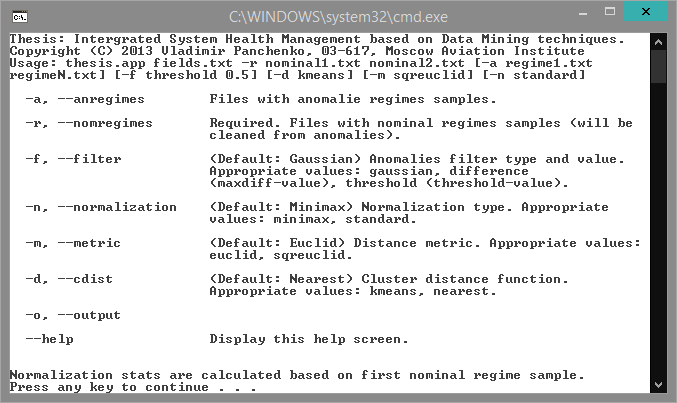
\includegraphics[width=0.7\textwidth]{scr_app_help}
\caption{Экран со справочной информацией}
\label{fig:spec:scr:AppHelp}
\end{figure}

\subsubsection{Работа с программным обеспечением}
Если все параметры для запуска были указаны корректно, программа запрашивает у пользователя ввод порогового значения $\varepsilon$, как показано на рисунке~\ref{fig:spec:scr:EnterEpsilon}.

\begin{figure}[h]
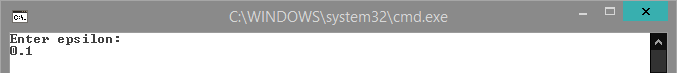
\includegraphics[width=0.7\textwidth]{scr_app_epsilon}
\caption{Ввод порогового значения в программу}
\label{fig:spec:scr:EnterEpsilon}
\end{figure}

После ввода программа отфильтровывает аномалии в указанных обучающих выборках и строит модель системы. Сначала выводятся найденные аномалии для указанных обучающих выборок номинальных режимов, а затем построенная база кластеров для каждого режима работы (рисунок~\ref{fig:spec:scr:SystemModel}).

\begin{figure}[h]
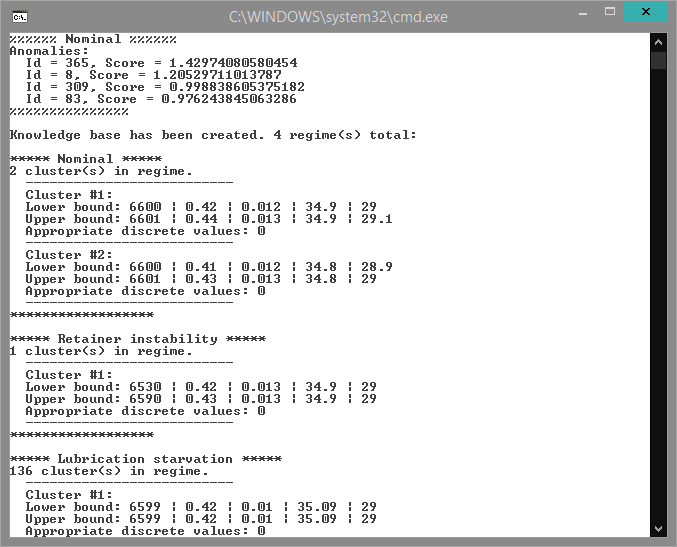
\includegraphics[width=0.7\textwidth]{scr_app_systemmodel}
\caption{Построенная программой модель системы}
\label{fig:spec:scr:SystemModel}
\end{figure}

После чего программа готова к мониторингу поступающих телеметрических данных, о чём сообщает пользователю соответствующим сообщением (рисунок~\ref{fig:spec:scr:EnterRecord}). Для выхода из режима мониторинга необходимо нажать \textit{Enter}.

\begin{figure}[h]
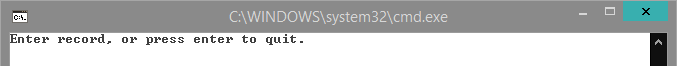
\includegraphics[width=0.7\textwidth]{scr_app_enterrecord}
\caption{Режим мониторинга: ввод записи}
\label{fig:spec:scr:EnterRecord}
\end{figure}

Записи вводятся в том же формате, что и во входных файлах. После ввода записи программа показывает результат мониторинга (текущий режим/текущий режим и расстояние до него/факт наличия аномалии, ближайший режим и расстояние до него). Пример работы программы в режиме мониторинга приведён на рисунке~\ref{fig:spec:scr:Monitoring}.

\begin{figure}[h]
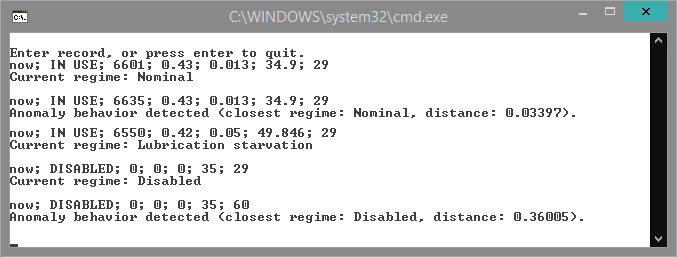
\includegraphics[width=0.7\textwidth]{scr_app_monitoring}
\caption{Режим мониторинга}
\label{fig:spec:scr:Monitoring}
\end{figure}

\section{Тестирование системы и анализ результатов}
Тестирование системы производилось на основе реальных данных телеметрии гиросилового комплекса управления Международной Космической Станции (МКС), собранных за период времени из~\cite{ISSLiveCMGConsole}. Важным фактом является то, что система, подобная разрабатываемой, уже применяется NASA для контроля и диагностики данной части МКС~\cite{IversonSHMforSpaceMissionOperations}.

Гиросиловой комплекс управления показан на рисунке~\ref{fig:spec:results:ISSCMGSystem}. Он состоит из четырёх гироскопов с управляющим моментом (гиродинов).

\begin{figure}[h]
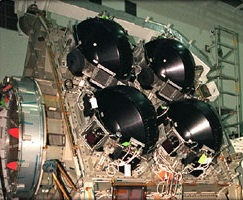
\includegraphics{iss_cmg_system}
\caption{Гиросиловой комплекс управления МКС}
\label{fig:spec:results:ISSCMGSystem}
\end{figure}

Так как характеристики гиродинов отличаются в зависимости от экземпляра~\cite{IversonSHMforSpaceMissionOperations}, контроль и диагностика с помощью методов интеллектуального анализа данных должна производиться для каждого гиродина по отдельности. Измеряемые параметры гиродина представлены в таблице~\ref{tab:spec:results:CMGParams}. Соответствующий им файл описания параметров представлен в листинге~\ref{lst:spec:results:params}.

\begin{table}[h]
\caption{Измеряемые параметры гиродина}
\label{tab:spec:results:CMGParams}
\begin{tabular}{|C{70pt}|C{250pt}|C{100pt}|}
\hline
Параметр & Описание & Единица измерения \\
\hline
$T$ & Дата и время измерения & дд/чч:мм:сс \\
\hline
$S$ & Состояние (используется/выключен из комплекса) & --  \\
\hline
$\omega$ & Скорость вращения ротора & об/мин \\
\hline
$I$ & Ток, потребляемый двигателем ротора & A \\
\hline
$a$ & Вибрация & g м/с\textsuperscript{2} \\
\hline
$t_b$ & Температура на креплении ротора & \textdegree C \\
\hline
$t_h$ & Температура на датчике скорости вращения & \textdegree C \\
\hline
\end{tabular}
\end{table}

\begin{algorithm}[h]
\caption{Файл с описанием параметров}
\label{lst:spec:results:params}
\raggedright
\addtolength{\leftskip}{5mm}
\smallskip
Дата и время : ignore \\
Состояние : IN USE, DISABLED \\
Скорость вращения ротора : continuous \\
Потребляемый двигателем ротора ток : continuous \\
Вибрация : continuous \\
Температура на креплении ротора : continuous \\
Температура на датчике скорости вращения : continuous \\
\end{algorithm}

Тестирование проводилось для четырёх известных режимов работы: двух штатных и двух нештатных. Данные по нештатным режимам взяты из~\cite{ISSCMGFailureAnalysis}~и~\cite{ISSCMGLessonsLearned}. Для удобства отображения данных для каждого режима было взято только 50 измерений. Для режима, когда гиродин выключен из комплекса, скорость вращения, вибрация и потребляемый ток равны нулю. Обучающие выборки приведены в приложении~\ref{app:Data}.

Штатные режимы:
\begin{itemize}
	\item номинальный (\textit{Nominal});
	\item гиродин выключен из комплекса (\textit{Disabled}).
\end{itemize}

Внештатные режимы:
\begin{itemize}
	\item нестабильность ретейнера ротора (\textit{Retainer instability});
	\item утечка смазки (\textit{Lubrication starvation}).
\end{itemize}

Графики изменения параметров для всех режимов показаны на рисунках~\ref{fig:spec:results:wheelspeed}--\ref{fig:spec:results:halltemp}. Как видно из графиков, в обучающей выборке для номинального режима присутствует аномалия измерения (запись №14).

\begin{figure}[h]
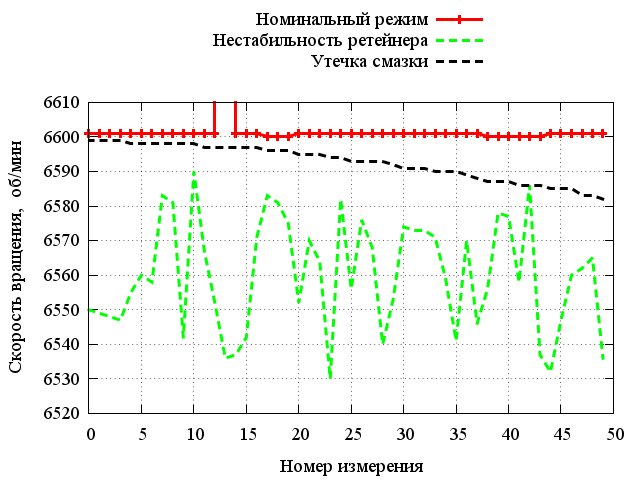
\includegraphics[width=0.7\textwidth]{results_wheelspeed}
\caption{Скорость вращения ротора для всех режимов работы гиродина}
\label{fig:spec:results:wheelspeed}
\end{figure}

\begin{figure}[h]
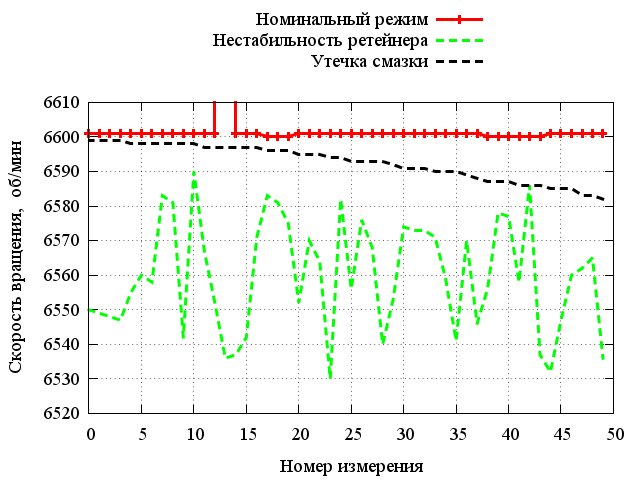
\includegraphics[width=0.7\textwidth]{results_wheelspeed}
\caption{Потребляемый двигателем ротора ток для всех режимов работы гиродина}
\label{fig:spec:results:current}
\end{figure}

\begin{figure}[h]
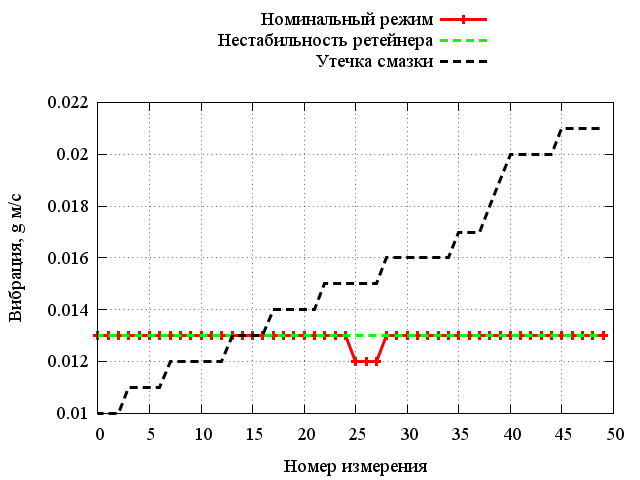
\includegraphics[width=0.7\textwidth]{results_vibration}
\caption{Вибрация для всех режимов работы гиродина}
\label{fig:spec:results:vibration}
\end{figure}

\begin{figure}[h]
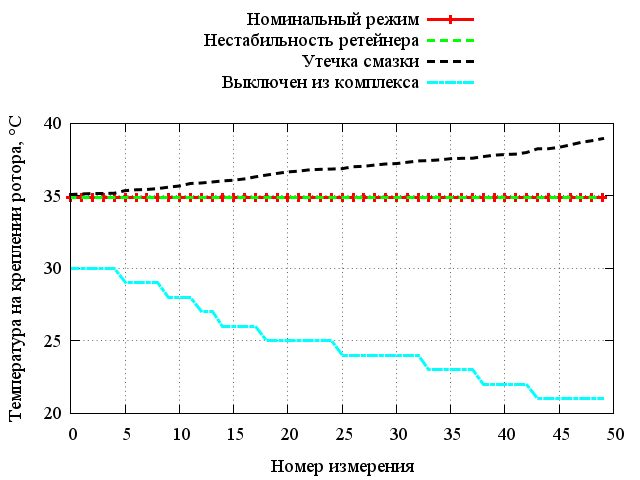
\includegraphics[width=0.7\textwidth]{results_wheeltemp}
\caption{Температура на креплении ротора для всех режимов работы гиродина}
\label{fig:spec:results:wheeltemp}
\end{figure}

\begin{figure}[h]
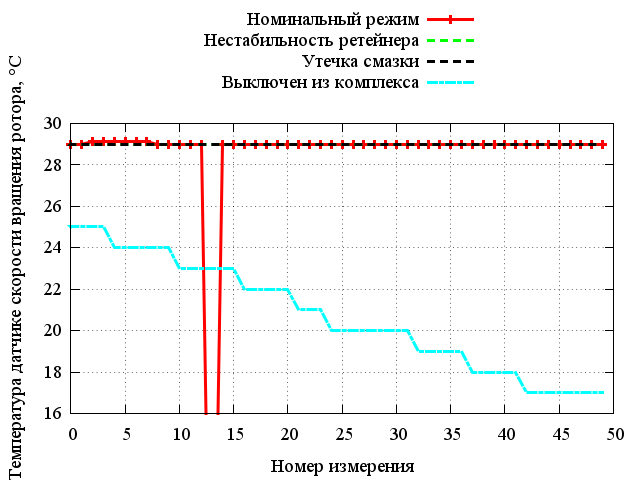
\includegraphics[width=0.7\textwidth]{results_halltemp}
\caption{Температура на датчике скорости вращения ротора для всех режимов работы гиродина}
\label{fig:spec:results:halltemp}
\end{figure}

Данные были загружены в систему. Использовались следующие настройки: пороговое значение $\varepsilon=0.05$, минимаксная нормализация, метрика расстояния по формуле~\eqref{eq:spec:DDMS:Distance}, расстояние до ближайшей точки кластера. Система корректно нашла аномалию в обучающей выборке для номинального режима работы (запись №14) и сформировала кластеры.

\begin{figure}
\caption{Модель ОК (номинальный режим работы)}
\label{fig:spec:results:scr:nominal}
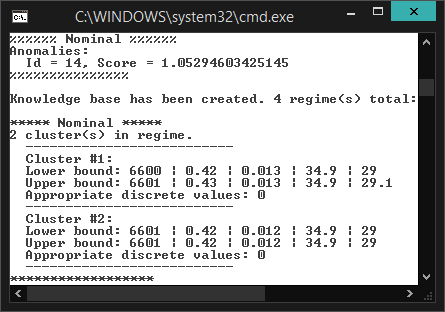
\includegraphics[width=0.6\textwidth]{results_scr_nominal}
\end{figure}

\begin{figure}
\caption{Модель ОК (гиродин выключен из комплекса)}
\label{fig:spec:results:scr:disabled}
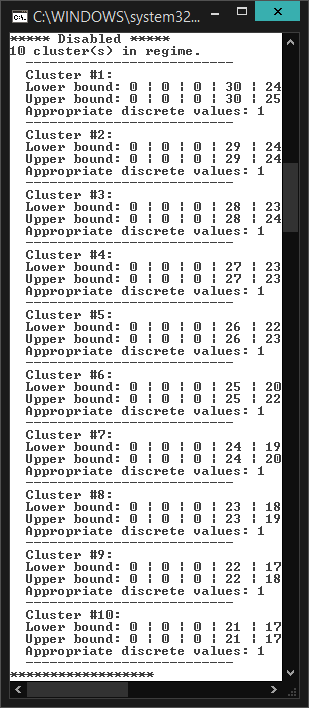
\includegraphics[height=0.6\textheight]{results_scr_disabled}
\end{figure}

\begin{figure}
\caption{Модель ОК (нештатные режимы)}
\label{fig:spec:results:scr:lubrret}
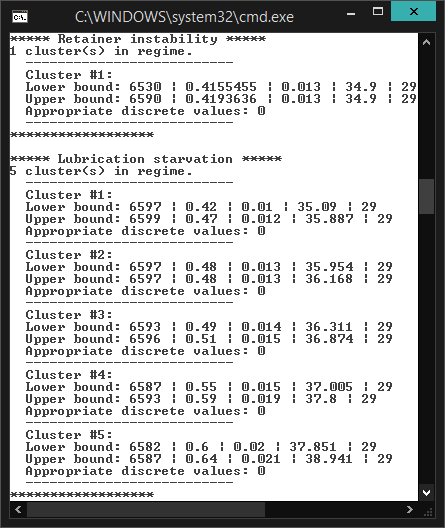
\includegraphics[width=0.5\textwidth]{results_scr_lubrret}
\end{figure}

Для проверки было взято несколько измерений, как относящихся к указанным режимам, так и заведомо аномальных (таблица~\ref{tab:spec:results:input}), и введены в систему. Результаты показаны на рисунке~\ref{fig:spec:results:monitoring}. Система не только верно определила состояние гиродина, но и показала степень отклонения и ближайший режим для аномальных измерений. Полученные результаты совпали с ожидаемыми.

Так как для обучения системы предполагается использовать большие массивы данных, был проведён нагрузочный тест. В качестве обучающей выборки для номинального режима были взяты данные телеметрии 335 дня с 18:17:16 по 20:37:57 и 338 дня с 13:42:23 по 19:50:00, вместе составляющие объём в 8437 записей. Время обработки данных составило 5 секунд, по результатам обучения система нашла 3 аномалии и создала 3 кластера для номинального режима работы. Результат показан на рисунке~\ref{fig:spec:results:scr:nominalFull}.

Таким образом, тестирование системы успешно завершено.

\begin{table}
\caption{Проверочные данные}
\label{tab:spec:results:input}
\begin{tabular}{|C{80pt}|C{50pt}|C{50pt}|C{50pt}|C{50pt}|C{50pt}|C{100pt}|}
\hline
$S$ & $\omega$ & $I$ & $a$ & $t_b$ & $t_h$ & Режим \\
\hline
IN USE & 6605 & 0.42 & 0.012 & 34.9 & 29 & Номинальный \\
\hline
DISABLED & 0 & 0 & 0 & 23 & 19 & Выключен из комплекса \\
\hline
IN USE & 6500 & 0.4 & 0.013 & 34.9 & 29 & Нестабильность ретейнера ротора \\
\hline
IN USE & 6590 & 0.55 & 0.015 & 37 & 29 & Утечка смазки \\
\hline
IN USE & 6500 & 0.6 & 0.02 & 42 & 31 & Аномалия \\
\hline
IN USE & 6601 & 0.42 & 0.012 & 24 & 10 & Аномалия \\
\hline
DISABLED & 6600 & 0.42 & 0.01 & 19 & 7 & Аномалия \\
\hline
\end{tabular}
\end{table}

\begin{figure}
\caption{Результаты мониторинга состояния ОК}
\label{fig:spec:results:monitoring}
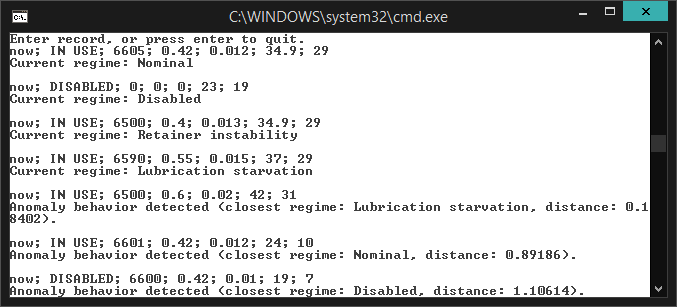
\includegraphics[width=0.7\textwidth]{results_monitoring}
\end{figure}

\begin{figure}
\caption{Результаты обучения системы на реальных данных}
\label{fig:spec:results:scr:nominalFull}
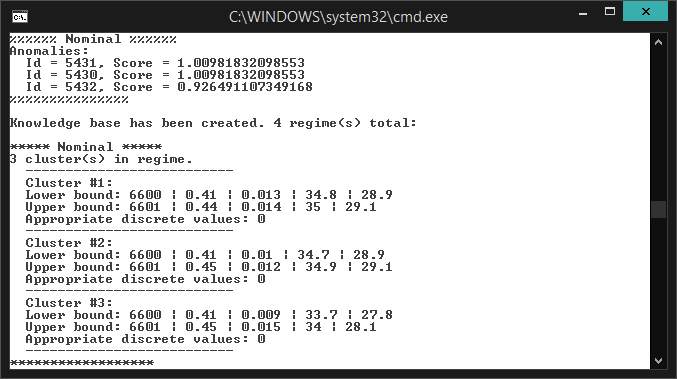
\includegraphics[width=0.7\textwidth]{results_scr_nominalFull}
\end{figure}